% ****** Start of file apssamp.tex ******
%
%   This file is part of the APS files in the REVTeX 4.2 distribution.
%   Version 4.2a of REVTeX, December 2014
%
%   Copyright (c) 2014 The American Physical Society.
%
%   See the REVTeX 4 README file for restrictions and more information.
%
% TeX'ing this file requires that you have AMS-LaTeX 2.0 installed
% as well as the rest of the prerequisites for REVTeX 4.2
%
% See the REVTeX 4 README file
% It also requires running BibTeX. The commands are as follows:
%
%  1)  latex apssamp.tex
%  2)  bibtex apssamp
%  3)  latex apssamp.tex
%  4)  latex apssamp.tex
%
\documentclass[%
  reprint,
  superscriptaddress,
%groupedaddress,
%unsortedaddress,
%runinaddress,
%frontmatterverbose,
%preprint,
%preprintnumbers,
%nofootinbib,
%nobibnotes,
%bibnotes,
  amsmath,amssymb,
  aps,
  prapplied,
%pra,
%prb,
%rmp,
%prstab,
%prstper,
%floatfix,
]{revtex4-2}

\usepackage{graphicx}% Include figure files
\usepackage{dcolumn}% Align table columns on decimal point
\usepackage{bm}% bold math
\usepackage{hyperref}% add hypertext capabilities
\hypersetup{
  colorlinks=true, % Set 'true' to enable colored links
  linkcolor=black, % Color of internal links (sections, pages, etc.)
  citecolor=black, % Color of citations
  filecolor=black, % Color of file links
  urlcolor=black, % Color of URL links
}
\usepackage{svg}
\usepackage{epstopdf}
\usepackage[utf8]{inputenc}
\usepackage[T1]{fontenc}
\usepackage{amsmath}
\usepackage{amsfonts}
\usepackage{amssymb}
%\usepackage[mathlines]{lineno}% Enable numbering of text and display math
%\linenumbers\relax % Commence numbering lines

%\usepackage[showframe,%Uncomment any one of the following lines to test
%%scale=0.7, marginratio={1:1, 2:3}, ignoreall,% default settings
%%text={7in,10in},centering,
%%margin=1.5in,
%%total={6.5in,8.75in}, top=1.2in, left=0.9in, includefoot,
%%height=10in,a5paper,hmargin={3cm,0.8in},
%]{geometry}
\usepackage{subcaption}
\usepackage{lipsum}

\begin{document}

\preprint{APS/123-QED}

\title{A coherently stimulated Brillouin spectrometer}

\author{Joel N. Johnson}
  \email{joel.johnson@nau.edu}
  \affiliation{Department of Applied Physics and Materials Science, Northern Arizona University, Flagstaff, AZ, 86011, USA}
  \affiliation{Center for Materials Interfaces in Research and Applications, Northern Arizona University, Flagstaff, AZ, 86011, USA}

\author{Co Authors}
  \affiliation{Department, Address}

\author{Ryan O. Behunin}
  \email{ryan.behunin@nau.edu}
  \affiliation{Department of Applied Physics and Materials Science, Northern Arizona University, Flagstaff, AZ, 86011, USA}
  \affiliation{Center for Materials Interfaces in Research and Applications, Northern Arizona University, Flagstaff, AZ, 86011, USA}

\date{\today}

\begin{abstract}
We present a novel coherently stimulated Brillouin spectrometer utilizing a detuned pump-probe design that exploits a relaxation of phase-matching requirements at small lengths, enabling room-temperature traveling-wave phonon spectroscopy at the micrometer scale with sub-10 femtowatt sensitivity. This approach overcomes the limitations of traditional stimulated Brillouin techniques, particularly regarding phase-matching constraints and spatial resolution. Our instrument's sensitivity was validated using 1 cm of UHNA3 fiber and 100 micrometers of bulk carbon disulfide liquid, demonstrating its capability to measure Brillouin scattering in materials with low Brillouin gain or, with particular advantage, small effective lengths. This advancement opens new possibilities for nanometer-scale Brillouin spectroscopy and the development of nano-acousto-optic devices.

%\begin{description}
%\item[Usage]
%Secondary publications and information retrieval purposes.
%\item[Structure]
%You may use the \texttt{description} environment to structure your abstract;
%use the optional argument of the \verb+\item+ command to give the category of each item.
%\end{description}
\end{abstract}

\keywords{Brillouin scattering, phonon spectrometer, phase-matching relaxation, nanometer-scale spectroscopy, photonics, femtowatt, pump-probe, instrument, room-temperature, nano-acousto-optic devices}%Use showkeys class option if keyword display desired

\maketitle

%\tableofcontents


\section{Introduction}
\label{sec:Introduction}

Brillouin scattering, the inelastic interaction between light and acoustic phonons, is a fundamental phenomenon used to probe the mechanical and structural properties of materials at microscopic scales. In spontaneous Brillouin scattering, thermally excited acoustic phonons scatter incident light, resulting in frequency shifts that reveal information about the material's elastic properties and acoustic modes \cite{boyd2020nonlinear}. However, the weak signal inherent to spontaneous Brillouin scattering often necessitates long acquisition times and limits spatial resolution, posing challenges for high-resolution material characterization.

Stimulated Brillouin scattering (SBS) enhances this interaction by using intense optical fields to amplify the acoustic wave through a nonlinear optical process. In SBS, a strong pump laser interacts with the counter-propagating Stokes wave generated within the medium, leading to the generation of acoustic phonons via electrostriction. This increased phonon population leads to greater generation of the Stokes wave, which interferes with the Pump wave to electrostrictively reinforce the acoustic wave. This positive feedback process creates exponential amplification that allows for more efficient excitation and detection of acoustic phonons and enables applications in optical signal processing, sensing, and high-resolution spectroscopy \cite{eggleton2013inducing, fotiadi2023brillouin, kobyakov2009stimulated, ippen1972stimulated}.

However, conventional SBS techniques face notable limitations when probing small volumes or samples with low Brillouin gain \cite{rakich2012giant, gyger2020observation}. The strict phase-matching conditions required for efficient SBS typically demand interaction lengths on the order of centimeters to meters, restricting spatial resolution and making it challenging to study micro- and nanoscale systems. Additionally, separating the pump and scattered signals often requires complex optical filtering due to their close spectral proximity, complicating the experimental setup.

To overcome these challenges, various approaches have been explored \cite{shin2013tailorable, van2015interaction, kittlaus2016large}. Techniques utilizing optical cavities enhance the interaction by increasing the effective interaction length, but they require precise alignment and are sensitive to environmental fluctuations \cite{pant2011cavity}. Forward Brillouin scattering methods, such as those demonstrated by Kittlaus et al., are advantageous in applications requiring relaxed phase-matching conditions, but come at the cost of increased modal complexity \cite{kittlaus2017chip}. Coherent probe beam amplification schemes have been proposed to improve sensitivity, yet they can introduce additional noise and complexity, as phase noise in laser sources can lead to significant gain fluctuations and performance penalties \cite{shlomovits2015effect}.

In this work, we present a coherently stimulated Brillouin spectrometer that employs a detuned pump-probe scheme to relax the phase-matching requirements at small interaction lengths. By introducing a separate probe laser detuned from the pump, we achieve coherent amplification of the acoustic wave without the need for strict phase-matching over long distances. This design allows for the separation of the probe and pump frequencies, simplifying signal detection and filtering.

Our approach enables room-temperature traveling-wave phonon spectroscopy at the micrometer scale with sub-10 femtowatt sensitivity, surpassing the limitations of traditional SBS techniques. We demonstrate the capabilities of our instrument by measuring Brillouin scattering in 1 centimeter of ultrahigh numerical aperture (UHNA3) fiber and 100 micrometers of bulk carbon disulfide liquid. These measurements highlight the instrument's ability to characterize materials with low Brillouin gain or small effective lengths.

The development of this coherently stimulated Brillouin spectrometer opens new avenues for nanometer-scale Brillouin spectroscopy and facilitates the characterization and development of nano-acousto-optic devices. It holds promise for advancing research in material science, photonics, and sensing technologies, where high spatial resolution and sensitivity are paramount, marking a significant step toward practical, room-temperature Brillouin-based spectroscopy and sensing solutions.

\section{Theoretical Framework}
\label{Theoretical Framework}

\subsection*{Coherently stimulated four-wave Brillouin scattering}
\label{Theoretical Framework:Coherently stimulated five-wave Brillouin scattering}
Stimulated Brillouin scattering (SBS), illustrated by the schematic in Fig. \ref{fig:4-Wave-Brillouin-Scattering}(a) for the Stokes process, is a three-wave mixing process in which incident pump laser light of frequency $\omega_{Pump}$ inelastically scatters from a traveling-wave phonon of frequency $\Omega$ to produce light that is frequency-shifted by the phonon frequency. In the Stokes process the phonon is retreating from the incident laser light and the scattered light is shifted down in frequency ($\omega_{Stokes} = \omega_{Pump} - \Omega$). Spatial overlap of the backscattered light with the incident laser light allows for interference of the two optical fields to produce a frequency at the difference of the two ($\omega_{Pump} - \omega_{Stokes}$). Since this difference frequency is exactly equal to the frequency of the acoustic field $\Omega$, the beating of the incident pump light with the backscattered Stokes light produces an electrostrictive reinforcement of the acoustic wave. This driving of the acoustic wave in turn increases the scattering rate of the incident pump light, producing a positive feedback process and an exponential increase of the amplitude of the backscattered Stokes wave.

\begin{figure*}[t]
  \centering
  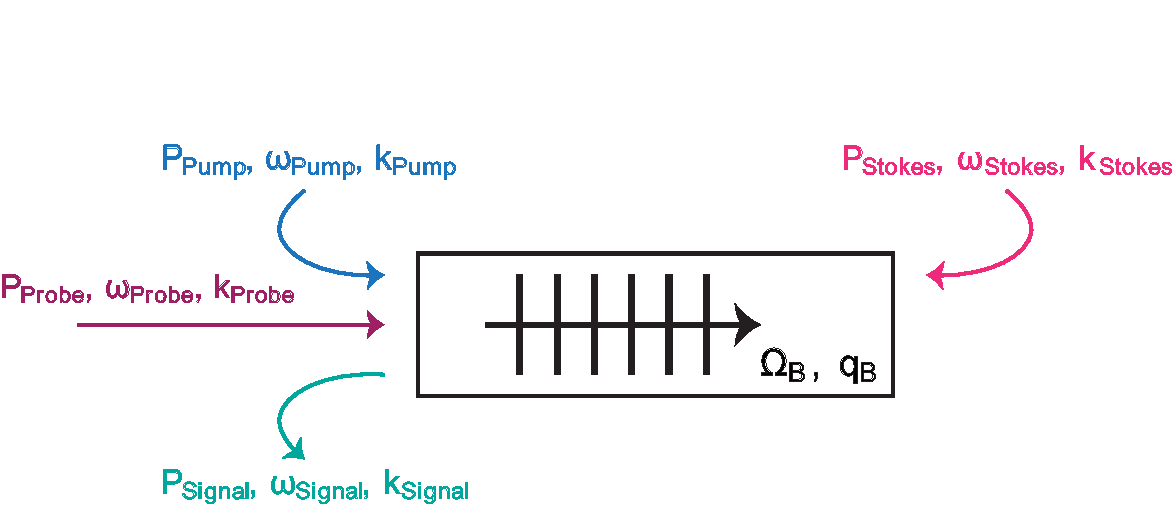
\includegraphics[width=.5\textwidth]{4-Wave-Brillouin-Scattering.pdf}
  \caption{Illustration of 4-Wave Brillouin Scattering.}
  \label{fig:4-Wave-Brillouin-Scattering}
\end{figure*}

Fig. \ref{fig:4-Wave-Brillouin-Scattering}(b) shows the schematic of coherently stimulated four-wave Brillouin scattering for the Stokes process. We introduce a strong, controlled external Stokes wave of frequency $\omega_{Stokes}$ that drives electrostrictive reinforcement of the acoustic field in the medium. The backscattered Stokes light, normally collected in an SBS process, is then drowned out by the external Stokes laser. To resolve this, we inject light of a distinct frequency $\omega_{Probe}$ from an additional external laser which copropagates with the Pump and backscatters in the medium from the strongly driven acoustic field. This produces backscattered Signal light to be collected ($\omega_{Signal} = \omega_{Probe} - \Omega$) which is spectrally distinct from the high-powered Stokes laser light.

To describe this interaction and characterize the performance of the instrument, we derive the coupled-wave equations for the four-wave mixing process in Appendix \ref{Appendix:Coupled-Wave Equations}. These equations describe the relationship between the optical fields and the acoustic field in the material and result in the following expression for the scattered power of the backscattered signal,
\\
\begin{equation}
  P_{Sig} = \frac{1}{4}(G_{B}L)^{2}P_{P}P_{S}P_{Pr}sinc^{2}\left(\frac{\Delta kL}{2}\right),
  \label{Eq:Theoretical Framework:Scattered Power} %compress sinc term into Psi here?
\end{equation}
\\
where $P_{P}$, $P_{S}$, and $P_{Pr}$ are the powers of the pump, Stokes, and probe lasers, respectively, and $G_{B}$ is the effective Brillouin gain,
\\
\begin{equation}
  G_{B} = \frac{g_{0}}{A_{eff}}\frac{\left(\frac{\Gamma_{B}}{2}\right)^{2}}{(\Omega - \Omega_{B})^{2} + \left(\frac{\Gamma_{B}}{2}\right)^{2}},
  \label{Eq:Effective Brillouin Gain}
\end{equation}
\\
with the on-resonance gain factor of the material given by
\\
\begin{equation}
  g_{0} = \frac{\gamma_{e}^{2}\omega^{2}}{nvc^{3}\rho_{0}\Gamma_{B}}.
\end{equation}
\\
Here, $\gamma_{e}$ is the electrostrictive constant, $\omega$ is the pump frequency, $n$ is the refractive index of the material, $v$ is the sound speed of the material, $c$ is the speed of light, $\rho_{0}$ is the mean density of the material, and $\Gamma_{B}$ is the Brillouin linewidth, or phonon dissipation rate, of the material. In Eq. \ref{Eq:Effective Brillouin Gain}, $\Omega_{B}$ is the resonant Brillouin frequency of the material, $A_{eff}$ is the effective area of the material, $\Delta k$ is the wavevector mismatch between the optical fields, to be discussed next, and $L$ is the effective length of the material.


\subsection*{Phase matching relaxation}
\label{Theoretical Framework: Phase matching relaxation}
In all nonlinear optical processes, efficiency is maximized when phase matching conditions are satisfied. A frequency mismatch (energy unconservation) or a wavevector mismatch (momentum unconservation) each result in drastically reduced efficiency of a given process.\cite{maker1962effects} This can be seen by Eq. \ref{Eq:Theoretical Framework:Scattered Power}, where the wavevector mismatch, $\Delta k$, is contained within a $sinc^{2}$ function. This $sinc^{2}$ term thereby defines the phase matching bandwidth of the system, notably scaling with effective interaction length $L$.

We apply this wavevector mismatch allowance to the pump and probe waves ($\Delta k = k_{Pump} - k_{Probe}$) so that the backscattered signal is different than the applied Stokes wave. This choice allows for selection of the signal and rejection of the Stokes with a bandpass filter, as will be discussed later. Expressed in terms of wavelengths, this gives
\\
\begin{equation}
  \Delta k = \frac{4\pi n\Delta\lambda}{\lambda_{Pump}\lambda_{Probe}} \approx \frac{4\pi n\Delta\lambda}{\lambda_{Pump}^{2}}.
\end{equation}
\\
We can apply this to the phasematching bandwidth term to find the fraction of maximum scattered power, $\Phi$, that can be expected for a given interaction length, $L$, and phase mismatch $\Delta\lambda$ between the pump and probe,
\\
\begin{equation}
  \Phi \equiv sinc^{2}\left(\frac{2\pi n\Delta\lambda L}{\lambda_{Pump}^{2}}\right).
  \label{Eq:Phi}
\end{equation}
\\
Using this expression for $\Phi$, we see that for an effective length of one meter, a wavelength mismatch of only 0.6 pm from a typical wavelength of 1.55 $\mu$m pump light in UHNA3 fiber drops the scattered power to one half of maximum. However, for shorter effective lengths the wavevector mismatch becomes more forgiving; a 36 pm mismatch preserves 82.5\% of the maximum signal for a length of 1 cm under identical conditions. This separation, translating to about 4.5 GHz, is meaningful, as it represents sufficient spectral separation for the backscattered signal to be isolated from the applied Stokes light.

Furthermore, for decreasing lengths, Eq. \ref{Eq:Phi} predicts an increase in the fraction of maximum signal produced, given equivalent pump-probe detuning, as the $sinc^{2}$ function is sampled closer to its peak center. Alternatively, as length decreases, the probe may be further detuned from the pump and still achieve the same fraction of the maximum signal as for longer lengths, perhaps offering a slight advantage in noise reduction. It should be noted that the scattered power, as given by Eq. \ref{Eq:Theoretical Framework:Scattered Power}, scales with the square of the effective length. Thus, while smaller lengths allow for the ability to capture a larger fraction of this maximum scattered power, the actual amount of scattered power decreases dramatically as length decreases.

\section{Methods}\label{Methods}
\subsection*{Instrument design}
\label{Methods:Instrument Design}

\begin{figure*}[htbp]
\centering
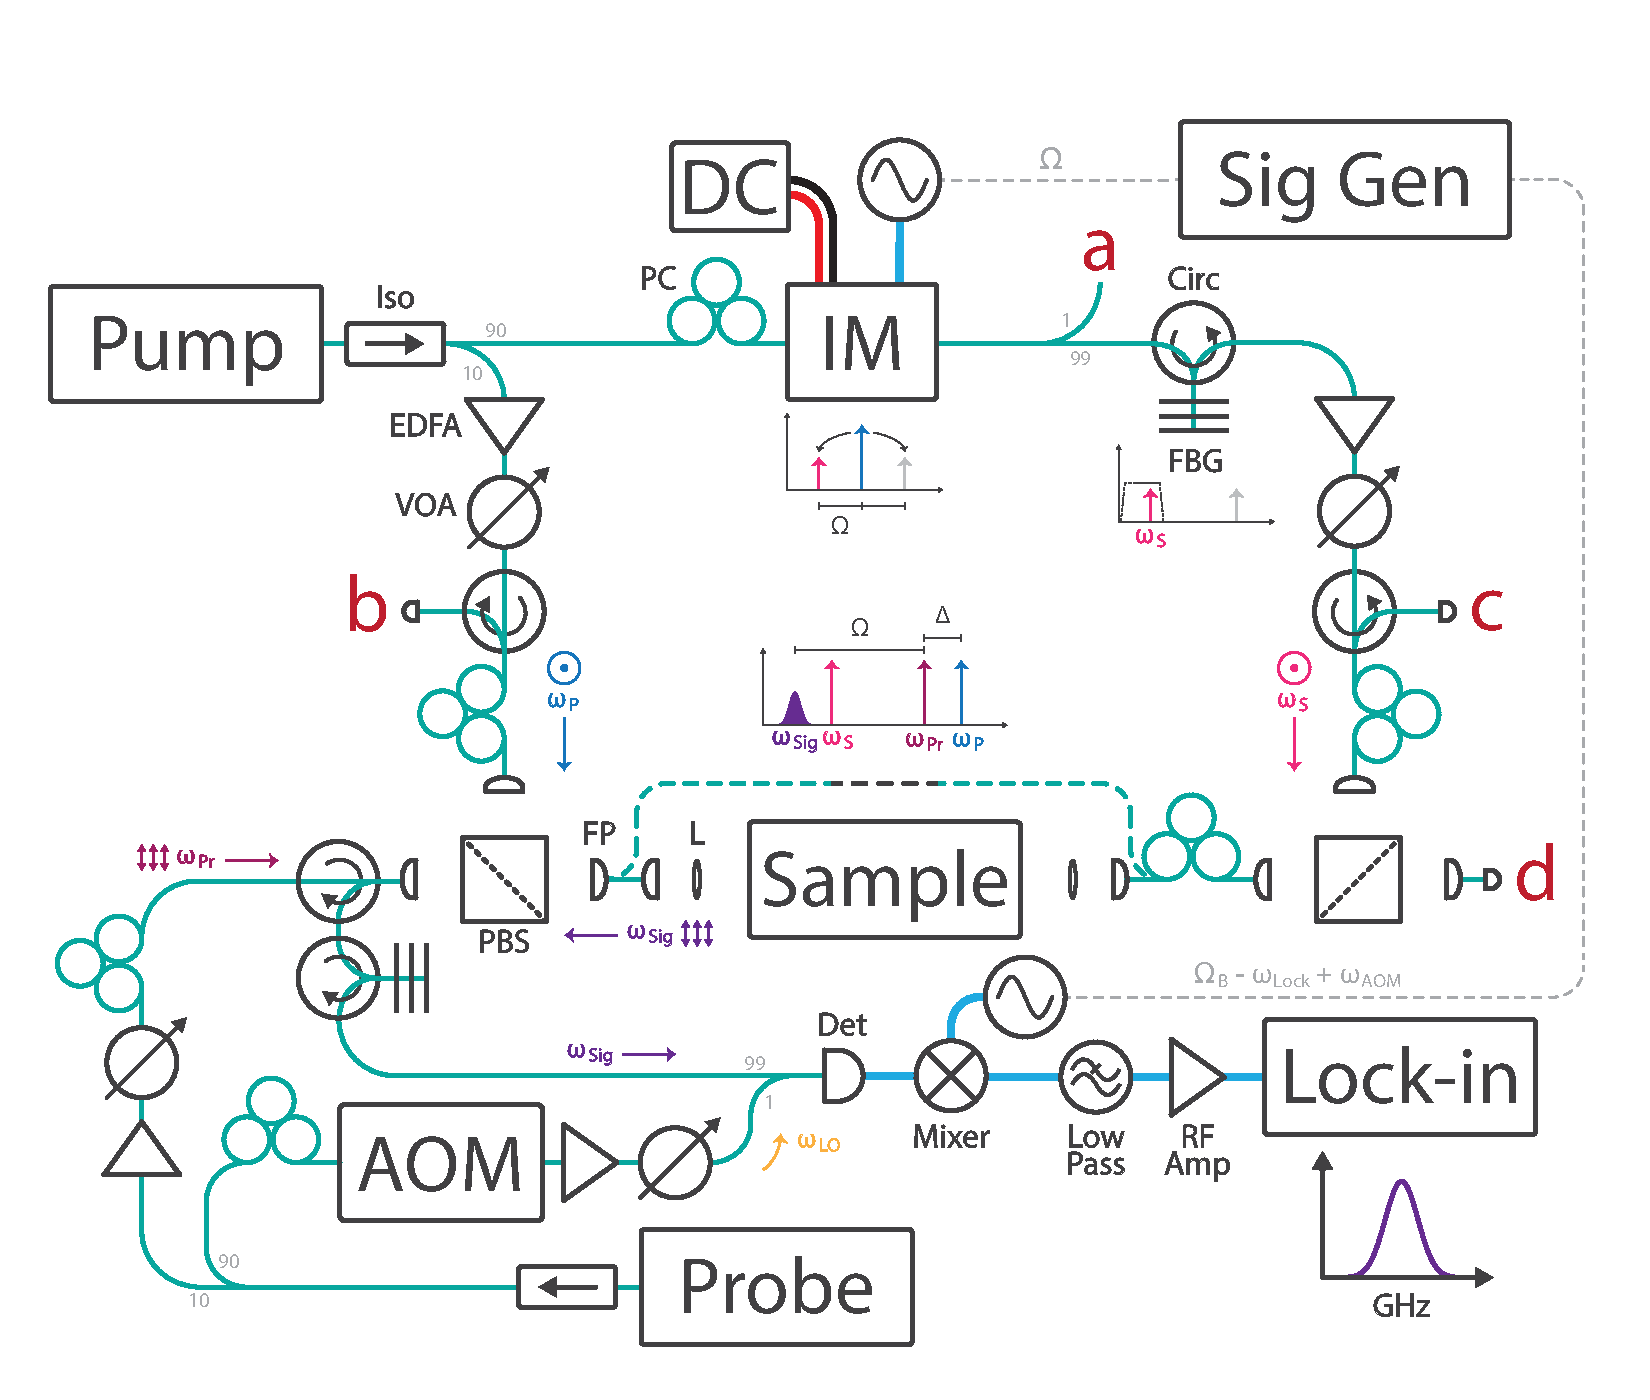
\includegraphics[width=\textwidth]{Instrument-Design-V1.pdf}
\caption{
Design schematic of a coherently stimulated phonon spectrometer. A tunable CW laser at approximately 1.55 $\mu$m emits light that passes through an isolator (Iso) and a splitter, diverting 10\% to a 27 dBm EDFA followed by a variable optical attenuator (VOA). This pump light ($\omega_P$) is polarization-controlled to reflect off a polarizing beam splitter (PBS) and is recoupled to fiber via a fiber port (FP), then directed to the sample either by direct fiber coupling or through a pair of FPs and lenses (L) for free-space samples. After passing through the sample, the pump light traverses a corrective polarization controller that mitigates fiber twists and bends before reflecting off a second PBS, where it is routed to port (c) for power monitoring. To synthesize the Stokes wave, a 90\% split from the original pump is processed through an intensity modulator (IM) and a fiber Bragg grating (FBG), generating a Stokes sideband downshifted from the pump by $\Omega$. This frequency shift is swept via a signal generator to capture $\Omega_B$. A 99/1 splitter provides a tap at port (a) to optimize Stokes synthesis. The Stokes wave ($\omega_S$), amplified by a 1 W EDFA and VOA-controlled, counter-propagates along the pump path and is monitored at port (b). A second tunable CW laser, detuned from the pump, generates the Probe wave ($\omega_{Pr}$), which is amplified by a 1 W EDFA, attenuated variably, and polarization-controlled to pass through the initial PBS where it is incident on the sample. Backscattered Signal light ($\omega_{sig}$) transmits back through the PBS, while unscattered Probe light transmits to a power meter at port (d). A circulator parts the Signal from the Probe path, with an FBG filtering out any unwanted noise or Stokes light. Finally, the Signal is heterodyned with an EDFA-amplified, AOM-shifted local oscillator (LO) derived from the Probe laser and directed to a photodiode for detection. The resulting RF signal is mixed with an AC LO supplied by the signal generator which sweeps synchronously with the Stokes synthesis frequency, and collected by a lock-in amplifier for data processing.
}
\label{fig:Instrument Design}
\end{figure*}

The design of the instrument is shown in the schematic in Fig. \ref{fig:Instrument Design}. A pump and Stokes wave is synthesized from a single tunable laser source for coherent stimulation of a sample. The pump wave ($\omega_{Pump}$) is amplified by an erbium-doped fiber amplifier (EDFA) and passed through a variable optical attenuator (VOA) for power control. The output is then polarization-controlled to reflect at a polarizing beam splitter (PBS) for injection into the sample. For Stokes synthesis, an AC signal ($\Omega$) is supplied to an intensity modulator (IM) with carrier frequency nulled and a tunable filter is used to select the lower-frequency Stokes side band ($\omega_{Pump} - \Omega$). This Stokes light is then amplified by an EDFA, passed through a VOA, and polarization-controlled to reflect at a second PBS for couter-propagation to the pump through the sample.

A separate tunable laser is used to supply a probe wave ($\omega_{Probe} = \omega_{Pump} + \Delta k$) and local oscillator (LO). Probe light is amplified by an EDFA and passed through a VOA and a polarization controller aligns the polarization for transmission through the first PBS whereby it copropagates with the pump through the sample. Backscattered light exits the sample and transmits back through the first PBS, whereas the orthogonally polarized Stokes light reflects at this same point to be diverted to a tap for power monitoring. The backscattered signal ($\omega_{Signal} = \omega_{Probe} - \Omega$) then routes through two subsequent circulators for spectral filtering by a 5 GHz bandpass tunable filter. This filter allows the desired backscattered signal to pass while rejecting any reflected probe light as well as any reflected, transmitted, or backscattered light from the pump or Stokes waves that was not already diverted by the PBS.

The filtered signal then heterodynes via a 99-1 splitter with the LO which is frequency-upshifted by an acousto-optic modulator (AOM) ($\omega_{LO} = \omega_{Probe} + \omega_{AOM}$) and controlled to be copolarized with the signal. Of the resulting frequencies from the heterodyne process, only the difference frequency term is considered, as all others are beyond the range of detection. This heterodyned signal ($\omega_{signal} = \Omega + \omega_{AOM}$) is then captured by a photodiode detector and heterodyned again by a radio frequency (RF) mixer with a second AC signal ($\Omega + \omega_{AOM} - \omega_{Lock}$), where $\omega_{Lock}$ is a fixed-frequency to be detected by a lock-in amplifier set to this frequency after being passed through a low-pass filter and amplified by an RF amplifier. Synchronous sweeping of both AC signals, each involving $\Omega$, allows for $\omega_{Lock}$ to remain fixed throughout measurement over a frequency range.

\subsection*{Experimental Techniques}
\label{Methods:Experimental Techniques}
Here we detail some of the experimental techniques, design choices, and specific device settings which optimize the signal-to-noise (SNR) of our measurements with the instrument. Our experimental setup generates the pump, Stokes, and Probe optical fields required for coherently stimulated Brillouin scattering. The pump laser emits approximately 45 mW of power, of which 10\% is split and amplified to approximately 0.5 W to become the pump optical field. The other 90\% of power emitted from the pump laser is shifted to become the Stokes optical field and is amplified to approximately 1 W. Similarly, the Probe laser emits approximately 45 mW of power, of which 10\% is split and amplified to approximately 1 W to become the Probe optical field and the remaining 90\% is used as the LO. A 99/1 splitter was specifically chosen over a more common 50/50 splitter to heterodyne the signal and LO in order to minimize loss of the backscattered signal before being collected by the detector, as this preserves 99\% of the signal power at no cost if the LO is amplified by 50x. Thus, in our setup the LO is amplified to approximately 230 mW prior to combining with the signal, resulting in the maximum allowable input power for our detector of <2.4 mW to be incident at the detector. Post-detector, the electronic signal is mixed with a 17 dbm AC signal and amplified by a 23 dbm RF amplifier before it is collected by a lock-in amplifier. For all measurements, it was found that setting both pump and Probe lasers to emit in whisper mode (as opposed to dither) dramatically improves the spectral density and SNR of the measurement.

Proper matching of the demodulator settings of our Zurich Instruments HF2LI 50 MHz lock-in amplifier to the signal input is critical for maximizing the SNR of the measurement. Clock timing is synced between the signal generater and the lock-in amplifier with a 10 MHz reference signal output from the signal generator and fed into the lock-in amplifier set to accept this reference clock signal. The input signal range, which defines the gain of the analog input amplifier, should exceed the incoming signal by roughly a factor two including a potential DC offset. This is best chosen by selecting the auto feature within the lock-in software interface, which automatically adjusts the range according to a rolling 100 ms window of the maximum measured input signal amplitude. The coupling mode is set to AC, which inserts a high-pass filter that rejects DC components of the input signal, and the input impedance is set to 1M$\Omega$. We set the low-pass filter order to the 8th order, which sets the filter to roll off at the maximum 48 dB/oct, and the data sampling rate of the input signal is set to the maximum 1.84 million Sa/s.

The SNR of a measurement is further optimized when the low-pass filter bandwidth for the lock-in amplifier input signal is minimized to match the frequency linewidth and thermally-driven variability or random drift of the incoming signal, $\omega_{Lock}$. While the linewidth of the signal is sub-hertz, the range within which it drifts is dependent on the stability of instrument components and is typically on the order of tens of hertz. We find this frequency drift of the input signal to be less than 100 Hz after all components of the system reach equilibrium temperature (approximately 30 minutes) and thus set the low-pass filter bandwidth to 100 Hz for long measurements of a few hours. For shorter measurements of less than 15 minutes this bandwidth can typically be reduced to as little as 40 Hz without risking the signal drifting out of range.

In addition to the signal linewidth being defined by this slight signal variability just discussed, the input signal frequency is also affected by the thermally-driven variations in precision of the electronic components. The mean frequency of the incoming signal, $\omega_{Lock}$, must precisely match the frequency that the lock-in amplifier expects to recieve, as specified in its control parameters. Achieving maximum precision requires that the frequency difference between the two output signals of the signal generator, $\omega_{Ch1} = \Omega$ and $\omega_{Ch2} = \Omega - \omega_{Lock} + \omega_{AOM}$, precisely match the lock-in frequency specified for the lock-in amplifier. This presents a challenge because, while $\Omega$ is directly controlled to subhertz precision by the signal generator, $\omega_{AOM}$ varies according to the precision of our AOM device with nominal temperature fluctuations. Despite efforts to thermally ground the device for stability, our AOM has been found to initially shift its input signal by its specified value of 40 MHz, before gradually increasing its applied shift over approximately 30 minutes as the internal components of the device warm to equilibrium operating temperature. Once at thermal equilibrium, however, the device maintains a stable shift of the signal by 40,000,820 Hz $\pm$ 50 Hz, allowing for a stable mean lock-in frequency and a relatively narrow filter bandwidth of 100 Hz to capture the variability contribution of the AOM.

\section{Results}\label{Results}
\subsection*{Instrument sensitivity}
\label{Results:Instrument sensitivity and SBS comparison}

\begin{figure}[t]
  \centering
  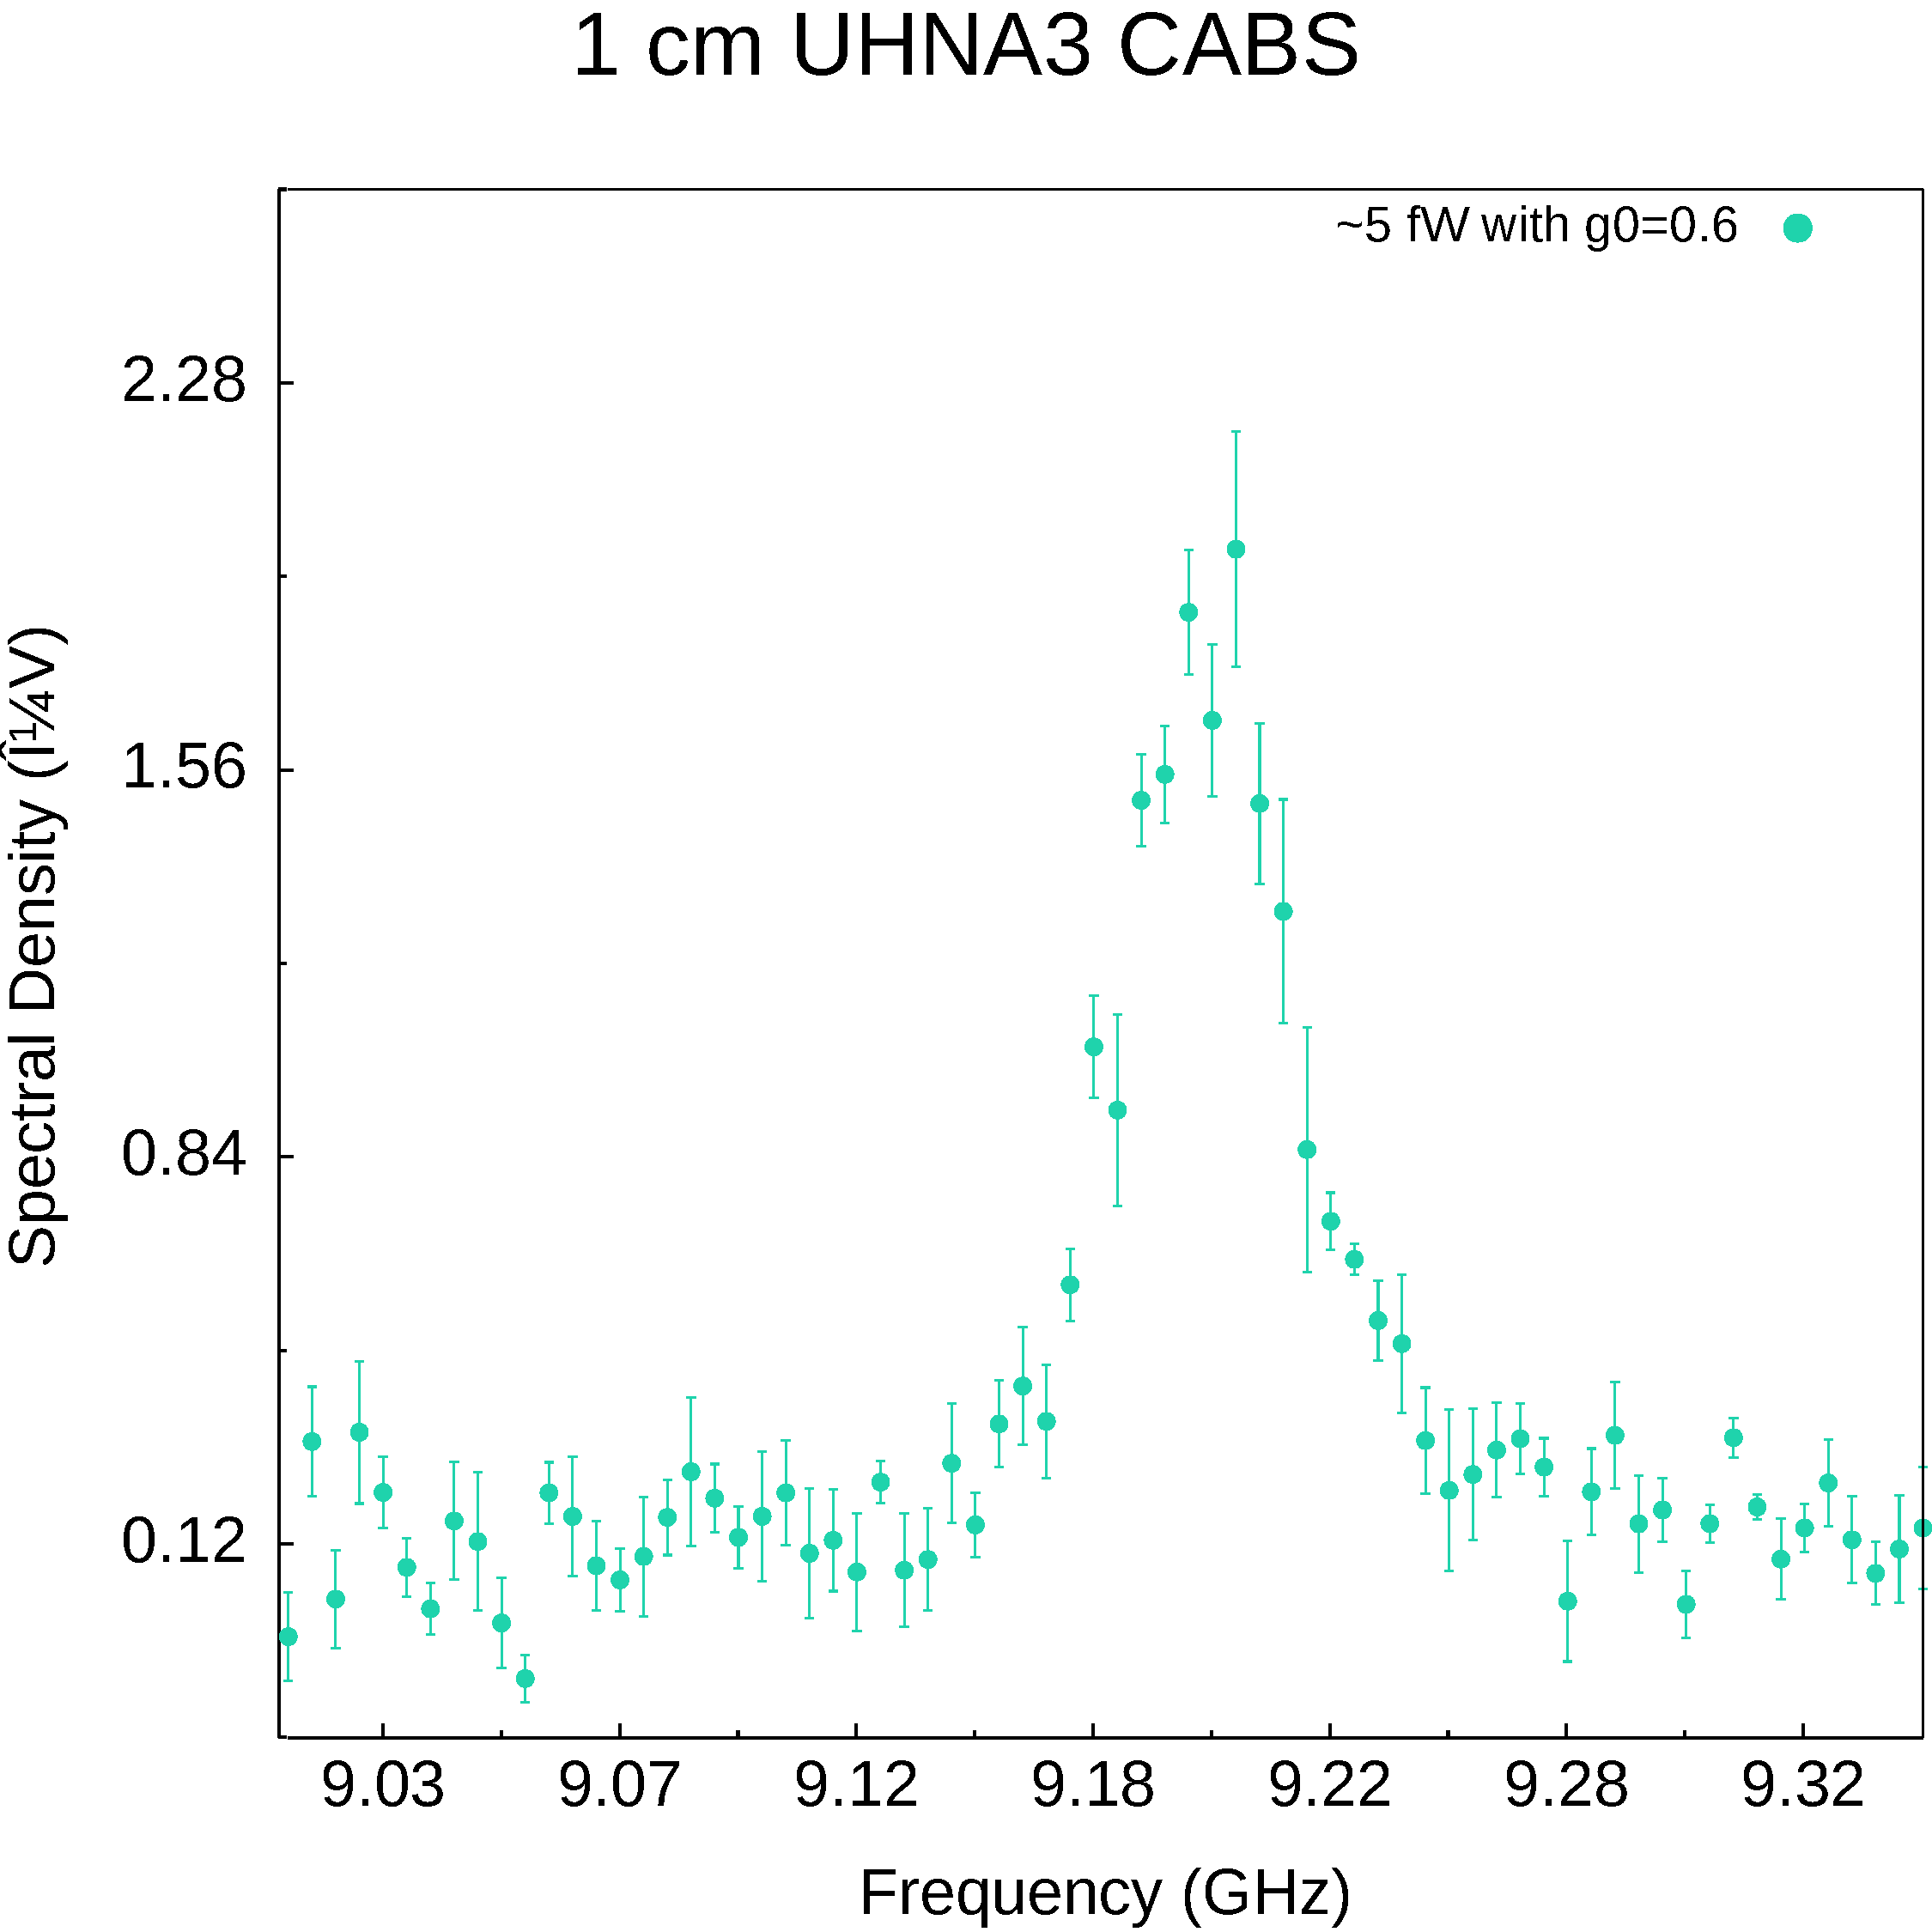
\includegraphics[width=.45\textwidth]{5fWSensitivity.pdf}
  \caption{~5 fW sensitivity measurement}
  \label{fig:5fWSensitivity}
\end{figure}

We begin by testing the sensitivity of the instrument as a way of defining a performance metric for the instrument which can be used to indicate what material, power, and length combinations might be possible to measure. From Eq. \ref{Eq:Theoretical Framework:Scattered Power}, the sensitivity of the instrument is the minimum scattered power, $P_{Signal}$, to produce a statistically significant measurement. To determine this, we target a specific length, $L$, of a sample of known effective Brillouin gain, $G_{B}$. We keep the pump-probe detuning, $\Delta\lambda$, constant across measurements and record the pump, Stokes, and probe optical powers to calculate the scattered power. Starting with sufficient optical powers to produce a clearly distinguishable measurement, we gradually reduce the optical powers until the sensitivity floor is reached.

To serve as our sensitivity testbed, we prepared 1 cm of Nufern's UHNA3 fiber, a well-studied fiber with known effective Brillouin gain\cite{behunin2015long}. Additionally, UHNA3 fiber offers several properties that make it ideal for this task of unambiguous detection of the Brillouin signal as it diminishes with each subsequent reduction in optical powers. First, it offers a Brillouin shift that is spectrally far from that of the single-mode fiber (SMF28) which constitutes much of the instrument. This ensures that the Brillouin response of the sample is not conflated with the Brillouin response of the instrument itself. Additionally, the core of UHNA3 fiber features a high concentration of germanium which improves the optical and acoustic guidance in the fiber as a result of the large refractive index difference between core and cladding. Finally, UHNA3 fiber offers a high optomechanical nonlinear response, with an effective Brillouin gain of 0.6 $W^{-1}m^{-1}$ measured at room temperature\cite{behunin2015long}. This gain factor is larger than that of SMF28 by an order of magnitude\cite{nikles1997brillouin}.

The Brillouin signal corresponding to a sensitivity of $P_{Signal}$ = 5\,fW is shown in Fig. \ref{fig:5fWSensitivity}. The data represent an average of five consecutive measurements, from which an average of five consecutive background measurements has been subtracted. Error bars indicate the $1\sigma$ standard deviation of the mean, also known as the standard error. The measurement appears to offer an SNR greater than 5, estimated by visually comparing the peak spectral density at the center frequency to the spectral density off resonance. Assuming a normal noise distrubution profile, an SNR of 5 is equivalent to a 5$\sigma$ confidence interval, or 99.7\% confidence in the statistical significance of this measurement. This characterization of the sensitivity of our instrument provides the essential information needed to assess the feasibility of more challenging measurements going forward, such as those involving materials with low Brillouin gain or samples with small effective lengths. Relevant parameters used for this measurement and calculation of on-resonance scattered power are listed in Table \ref{tab:sensitivity}.

\begin{table}[h]
    \centering
    \begin{tabular}{|c|c|c|c|c|c|}
        \hline
        $G_{B}$ & $L$ & $P_{P}$ & $P_{S}$ & $P_{Pr}$ & $\Delta\lambda$ \\
        $(W^{-1}m^{-1})$ & $(m)$ & $(\mu W)$ & $(\mu W)$ & $(mW)$ & $(pm)$ \\
        \hline
        0.6 & 0.01 & 506 & 504 & 2.01 & 20 \\
        \hline
    \end{tabular}
    \caption{Measurement parameters for sensitivity measurement and calculation.}
    \label{tab:sensitivity}
\end{table}

\subsection*{Measurements}
\label{Results:Measurements}

We demonstrate the capabilities of the instrument on the two most common classes of samples: fiber and bulk material. For a fiber sample we again choose UHNA3 for its higher nonlinear response and excellent optical and acoustic guidance. In contrast to the sensitivity measurements, we now seek to demonstrate the full measuring capabilities of the instrument and so apply all available optical power (about 1.5 W) to maximize the backscattered signal from the sample. We target the same 1 cm segment of UHNA3 fiber as was used for determining sensitivity.

\begin{figure}[t]
  \centering
  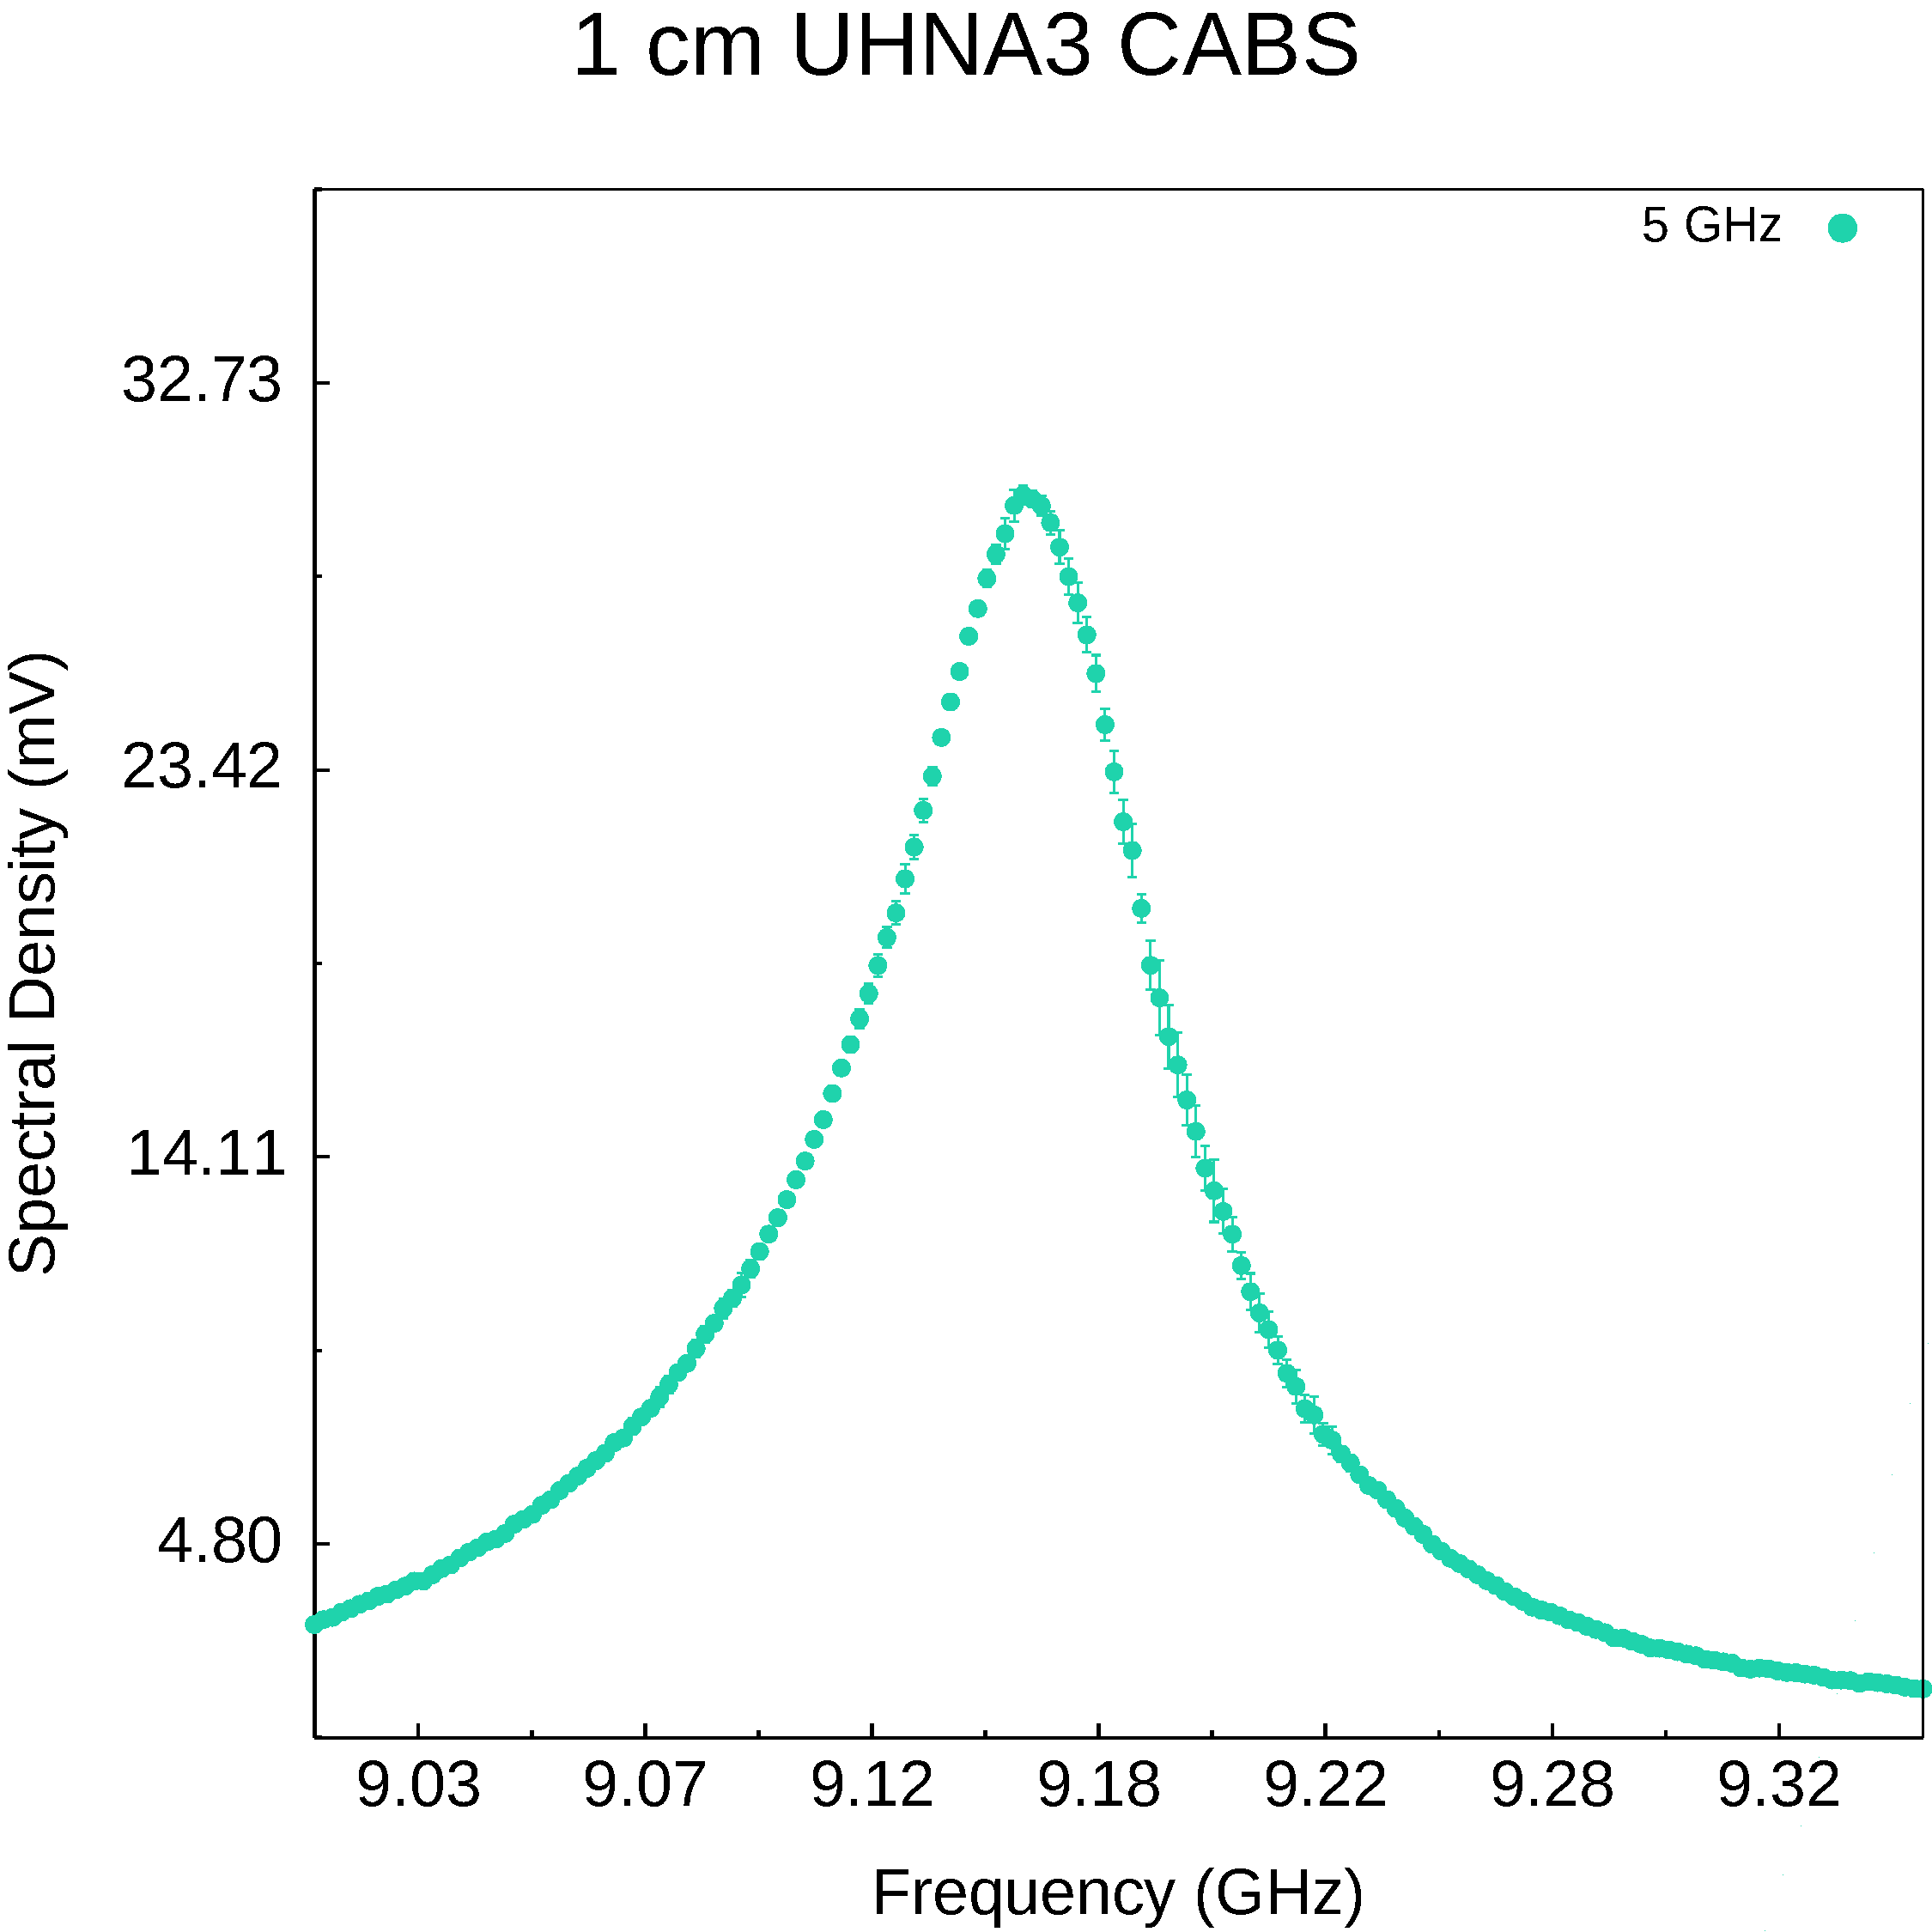
\includegraphics[width=.45\textwidth]{1cmUHNA3.pdf}
  \caption{1cm UHNA3}
  \label{fig:1cmUHNA3}
\end{figure}

Fig. \ref{fig:1cmUHNA3} shows the spectral profile captured for 1 cm of UHNA3 fiber, revealing the expected lorentzian profile consistent with Eq. \ref{Eq:Effective Brillouin Gain}. The peak amplitude of the spectra occurs at 9.1704 GHz, indicating the Brillouin resonance frequency of the longitudinal traveling-wave mode in the fiber. The FWHM of the measurement is 80 MHz and provides a measure of the phonon dissipation rate. Both values match what is seen in the literature for SBS measurements of UHNA3 fiber.\cite{behunin2015long} The data shown are a background-subtracted average of five successive measurements taken over 10 minutes with error bars corresponding to $1\sigma$ of the standard deviation of the mean, or standard error.

To achieve this measurement of UHNA3 fiber, the instrument design was altered to include only fiber-coupled segments connecting the fiber ports between the two PBSs. The pump laser wavelength was set to 1549.000 nm and the probe laser wavelength was set to 1549.020 nm, giving a frequency mismatch of approximately 2.5 GHz. The pump-probe mismatch is chosen to be only as large as needed to allow the edge of the pass-band of the probe filter to split the backscattered pump and probe light, thus rejecting any backscattered light from the pump laser and accepting only the backscattered signal from the probe laser. The Stokes filter was placed at 1549.073 nm, an offet of approximately 9.18 GHz from the pump laser to capture the Stokes sideband from the intensity modulator. This corresponds to the center of the measured frequency range and was chosen to allow the Stokes sideband output from the intensity modulator to remain within the pass band of the Stokes filter as the RF signal fed to the intensity modulator is swept through the full measurement range. The probe filter was set to 1549.109 nm, an offset of approximately 11.18 GHz from the probe laser, to capture the Stokes-shifted backscattered signal from the probe. The center frequency of the backscattered signal is of course shifted 9.18 GHz from the probe laser, however an extra offset of 2 GHz is chosen for improved rejection of any pump light as the pass band of our filter extends approximately 2.5 GHz on either side of center.

\begin{figure}[t]
  \centering
  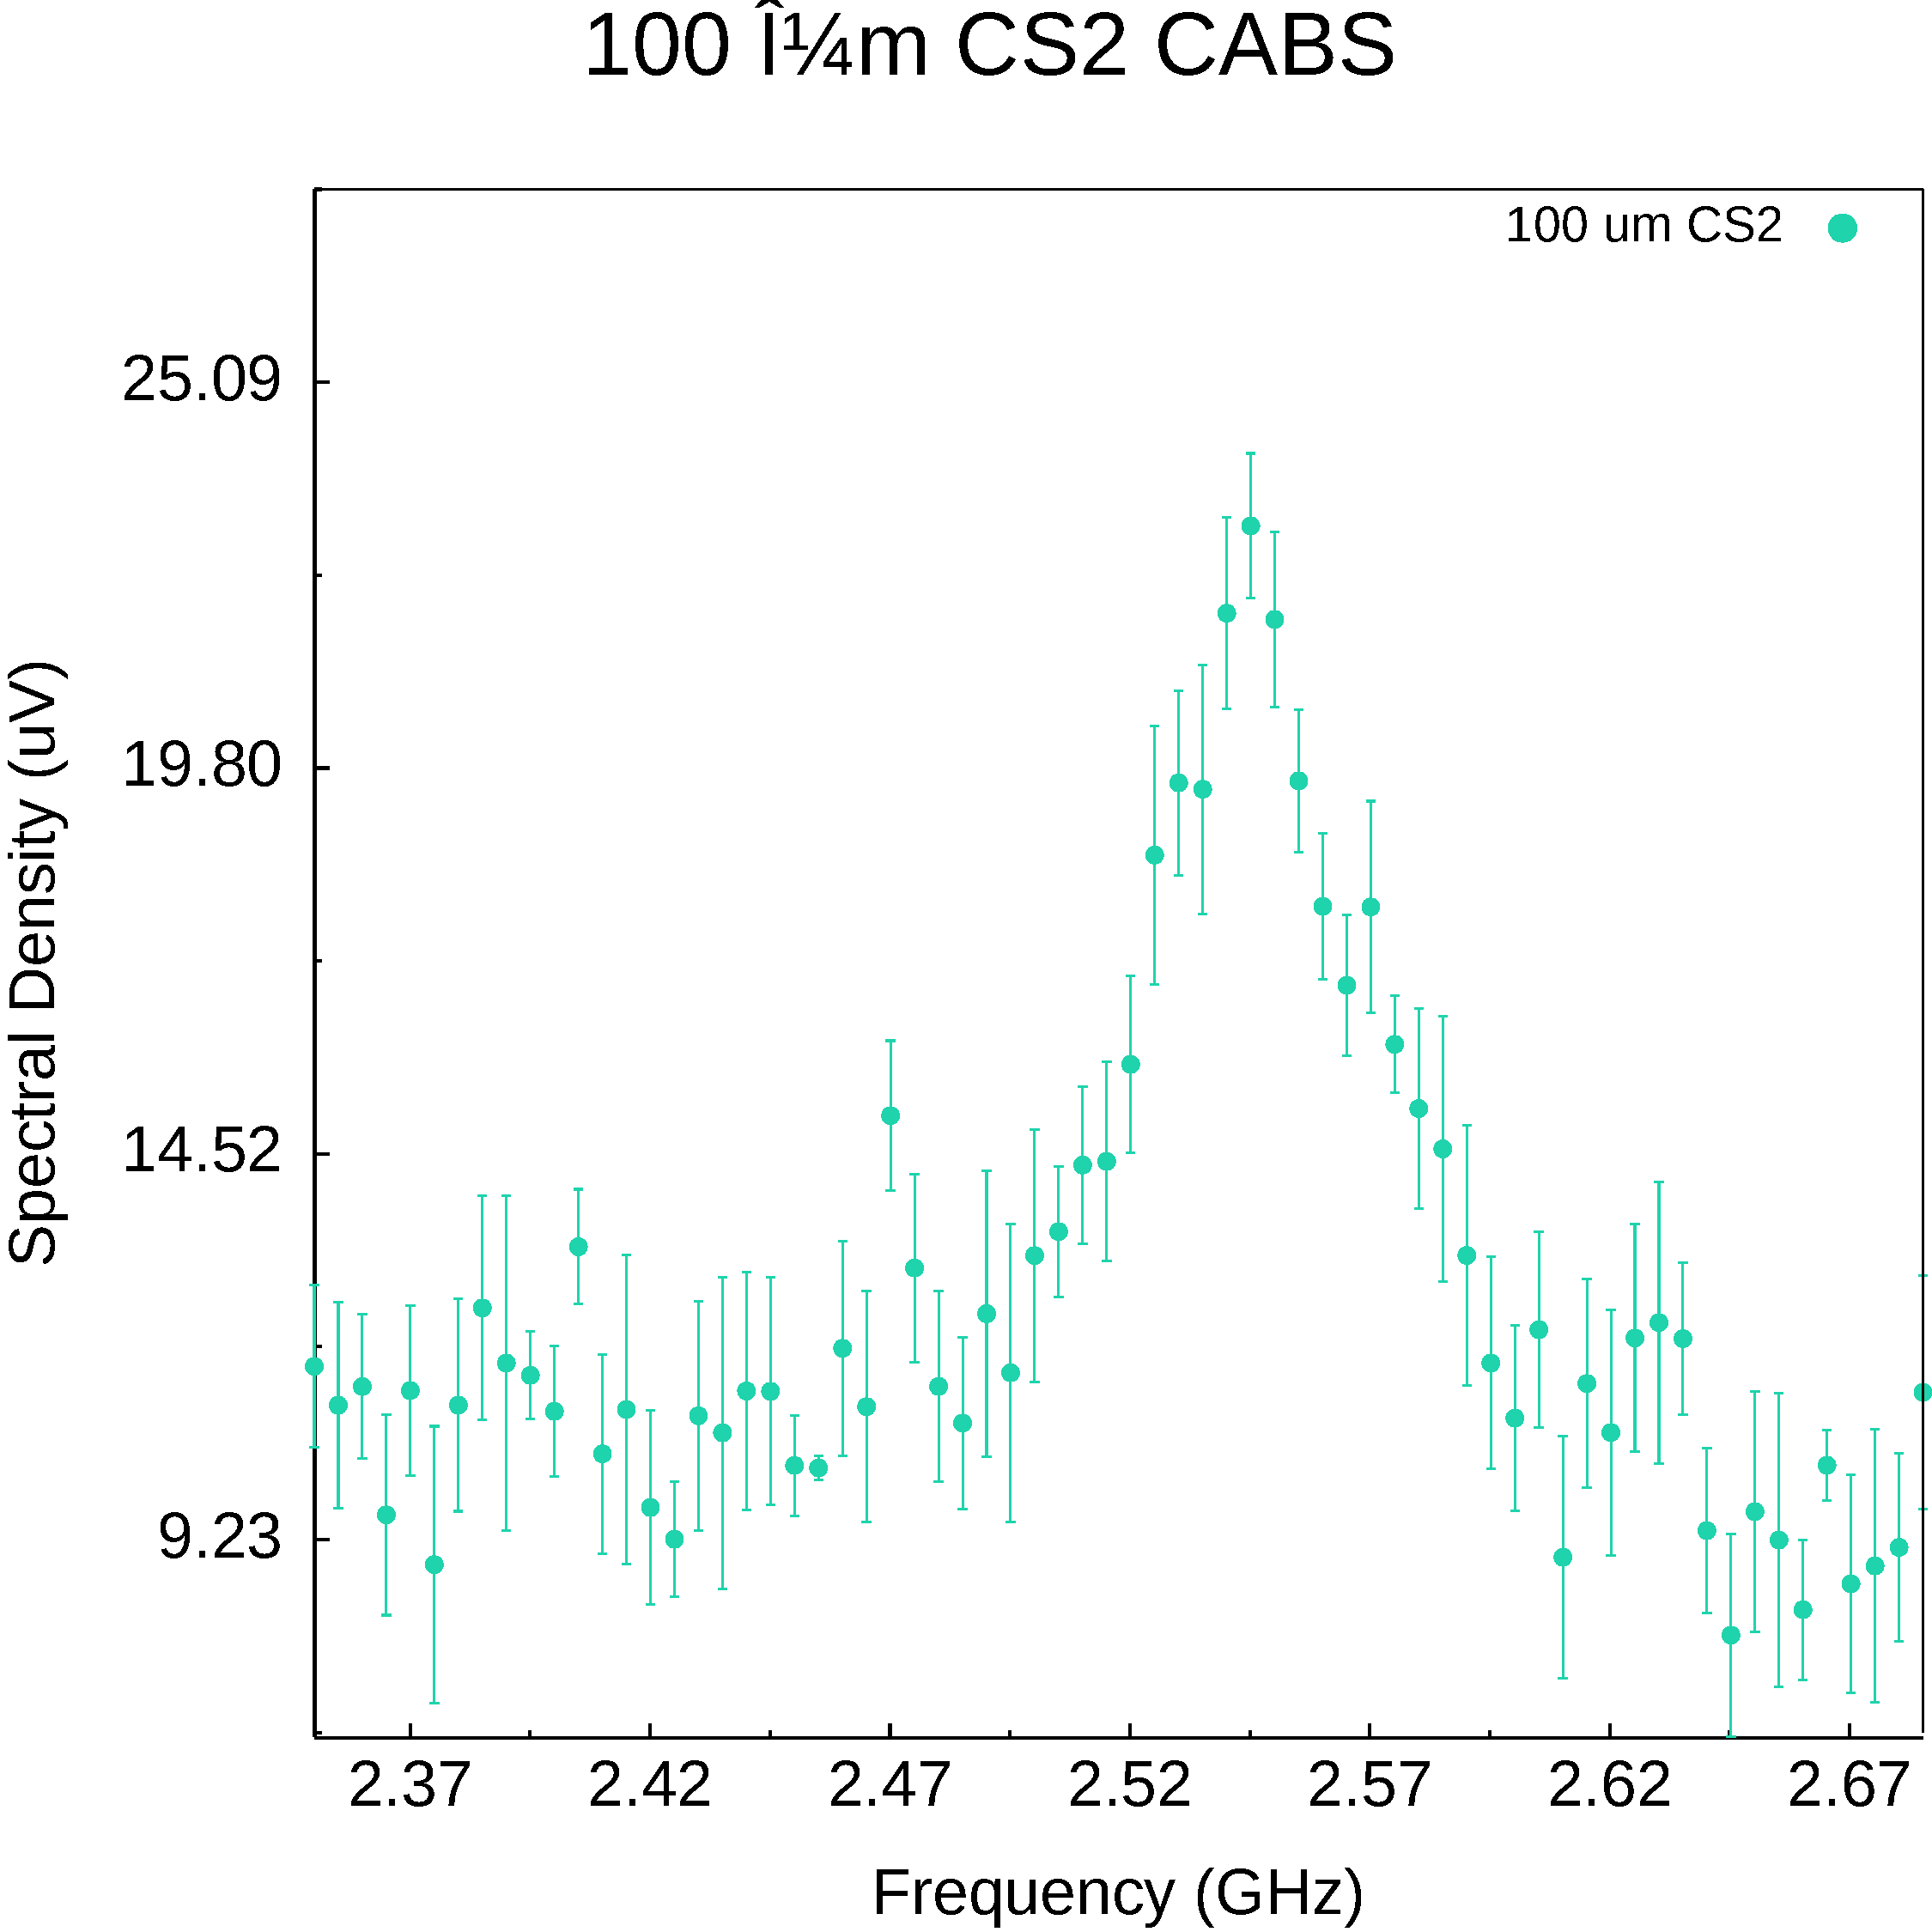
\includegraphics[width=.45\textwidth]{100umCS2.pdf}
  \caption{100$\mu$m CS2}
  \label{fig:100umCS2}
\end{figure}

For a free-space bulk example we target carbon disulfide liquid for its exceptionally high Brillouin gain factor of 1.5 m/GW.\cite{boyd2020nonlinear} Figure \ref{fig:100umCS2} reveals the Brillouin signal of carbon disulfide liquid contained in a 100 $\mu$m path length cell. To our knowledge, measurement of Brillouin scattering at this scale has not been reported in the literature. A scattered power comparison would reveal that achieving such a measurement using traditional SBS techniques would require excessively high optical powers or cooling the material to cryogenic temperatures, which, of course, would be prohibitive for carbon disulfide in the liquid state.

For this measurement of carbon disulfide, the pump and probe laser wavelengths were set to 1548.808 nm and 1548.898 nm, respectively. The short path length of the sample significantly broadens $\Phi$, the $sinc^{2}$ term defining the phasematching bandwidth, allowing for further separation of the pump and probe wavelengths for improved signal isolation without significant reduction in scattered power of the signal produced in the carbon disulfide. Specifically, the additional pump-probe wavelength separation of 70 pm employed for this measurement compared to the UHNA3 measurement results in a negligible 0.045\% reduction in scattered power. This additional separation contributes meaningfully, however, to improved rejection of pump light by the probe filter and thus higher SNR of the signal.

Placement of the Stokes filter is critical for measurements of materials that give small Brillouin shifts, such as with carbon disulfide's 2.55 GHz shift. We offset our 5GHz bandwidth Stokes filter an additional 2 GHz to ensure the nearby carrier signal and anti-Stokes sideband from the intensity modulator are rejected and only the Stokes sideband is allowed to pass. For the measurement shown in Fig. \ref{fig:100umCS2}, this corresponds to a Stokes and probe filter placement of 1548.844 nm and 1548.934 nm, respectively.

% Fig. shows the spectral measurements achieved by the instrument, overlaid with finite-difference simulation data. In Fig. we see the expected lorentzian spectral shape in good alignment with simulation data for guided longitudinal modes in the core of the UHNA3 fiber. In Fig. , however, we see a distortion of this lorentzian shape. This is expected for partially unguided longitudinal modes, such as is the case for a bulk liquid filling the volume of a ...
%
% Fig. \ref{fig:1cmUHNA3} shows a measurement of 1cm of UHNA3 fiber.
%
% First, we measured Brillouin scattering in a 1-centimeter-long UHNA3 fiber at room temperature and with sub-Watt optical power (Fig. ). Figure , clearly displays the Brillouin scattering features with remarkable SNR, highlighting the effectiveness of our apparatus in isolating the backscattered probe light. This observation serves as one of the main showcases of the instrument's capability.
%
% Next, we performed Brillouin scattering measurements on a 4-millimeter-thick bulk carbon disulfide sample in a free-space optics arrangement. The observed spectrum, presented in Figure 2, exhibits well-resolved Brillouin scattering peaks. This successful measurement in a bulk sample demonstrates the versatility and adaptability of our instrument to various experimental configurations, further emphasizing the instrument's capability.
%
% Lastly, we conducted a measurement in a 1-millimeter-long UHNA3 fiber under low-power conditions, with only 10 microwatts of power at the sample. Despite the reduced sample length and low power, the instrument's sensitivity allowed us to observe distinct Brillouin scattering features in the spectrum, as illustrated in Figure 3. This result underscores the potential of our spectrometer for nanoscale measurements and serves as a demonstration of the instrument's sensitivity, defining the sensitivity floor of the apparatus.
%
% These three observations collectively showcase the high sensitivity, broad applicability, and impressive capabilities of our coherent stimulated phonon spectrometer in measuring Brillouin scattering across different sample types, scales, and power levels.

\subsection*{Phase Matching Bandwidth}
\label{Results:Phase Matching Characterization}

We performed an additional experiment to characterize the phase matching tolerance of the instrument for a given length of sample. In this experiment, we performed a series of measurements of 1 cm of UHNA3 at constant optical powers while increasing the detuning of pump and probe lasers. From Eq. \ref{Eq:Theoretical Framework:Scattered Power}, this experiment holds $G_{B}$, $L$, $P_{P}$, $P_{S}$, and $P_{Pr}$ constant while letting $\Delta k$ vary. We expect the amplitudes of these measurements to trace out a $sinc^{2}$ function as given by Eq. \ref{Eq:Phi}. Fig. \ref{fig:Phase-Match} shows the result of this experiment which includes 75 measurements performed between 5 GHz and 42 GHz pump-probe frequency separation, at 0.5 GHz intervals, with the peak amplitude of each measurement represented by a point. The theoretical $sinc^{2}$ function for the parameters used in the experiment is shown on the plot with a solid red line.

\begin{figure}[t]
\centering
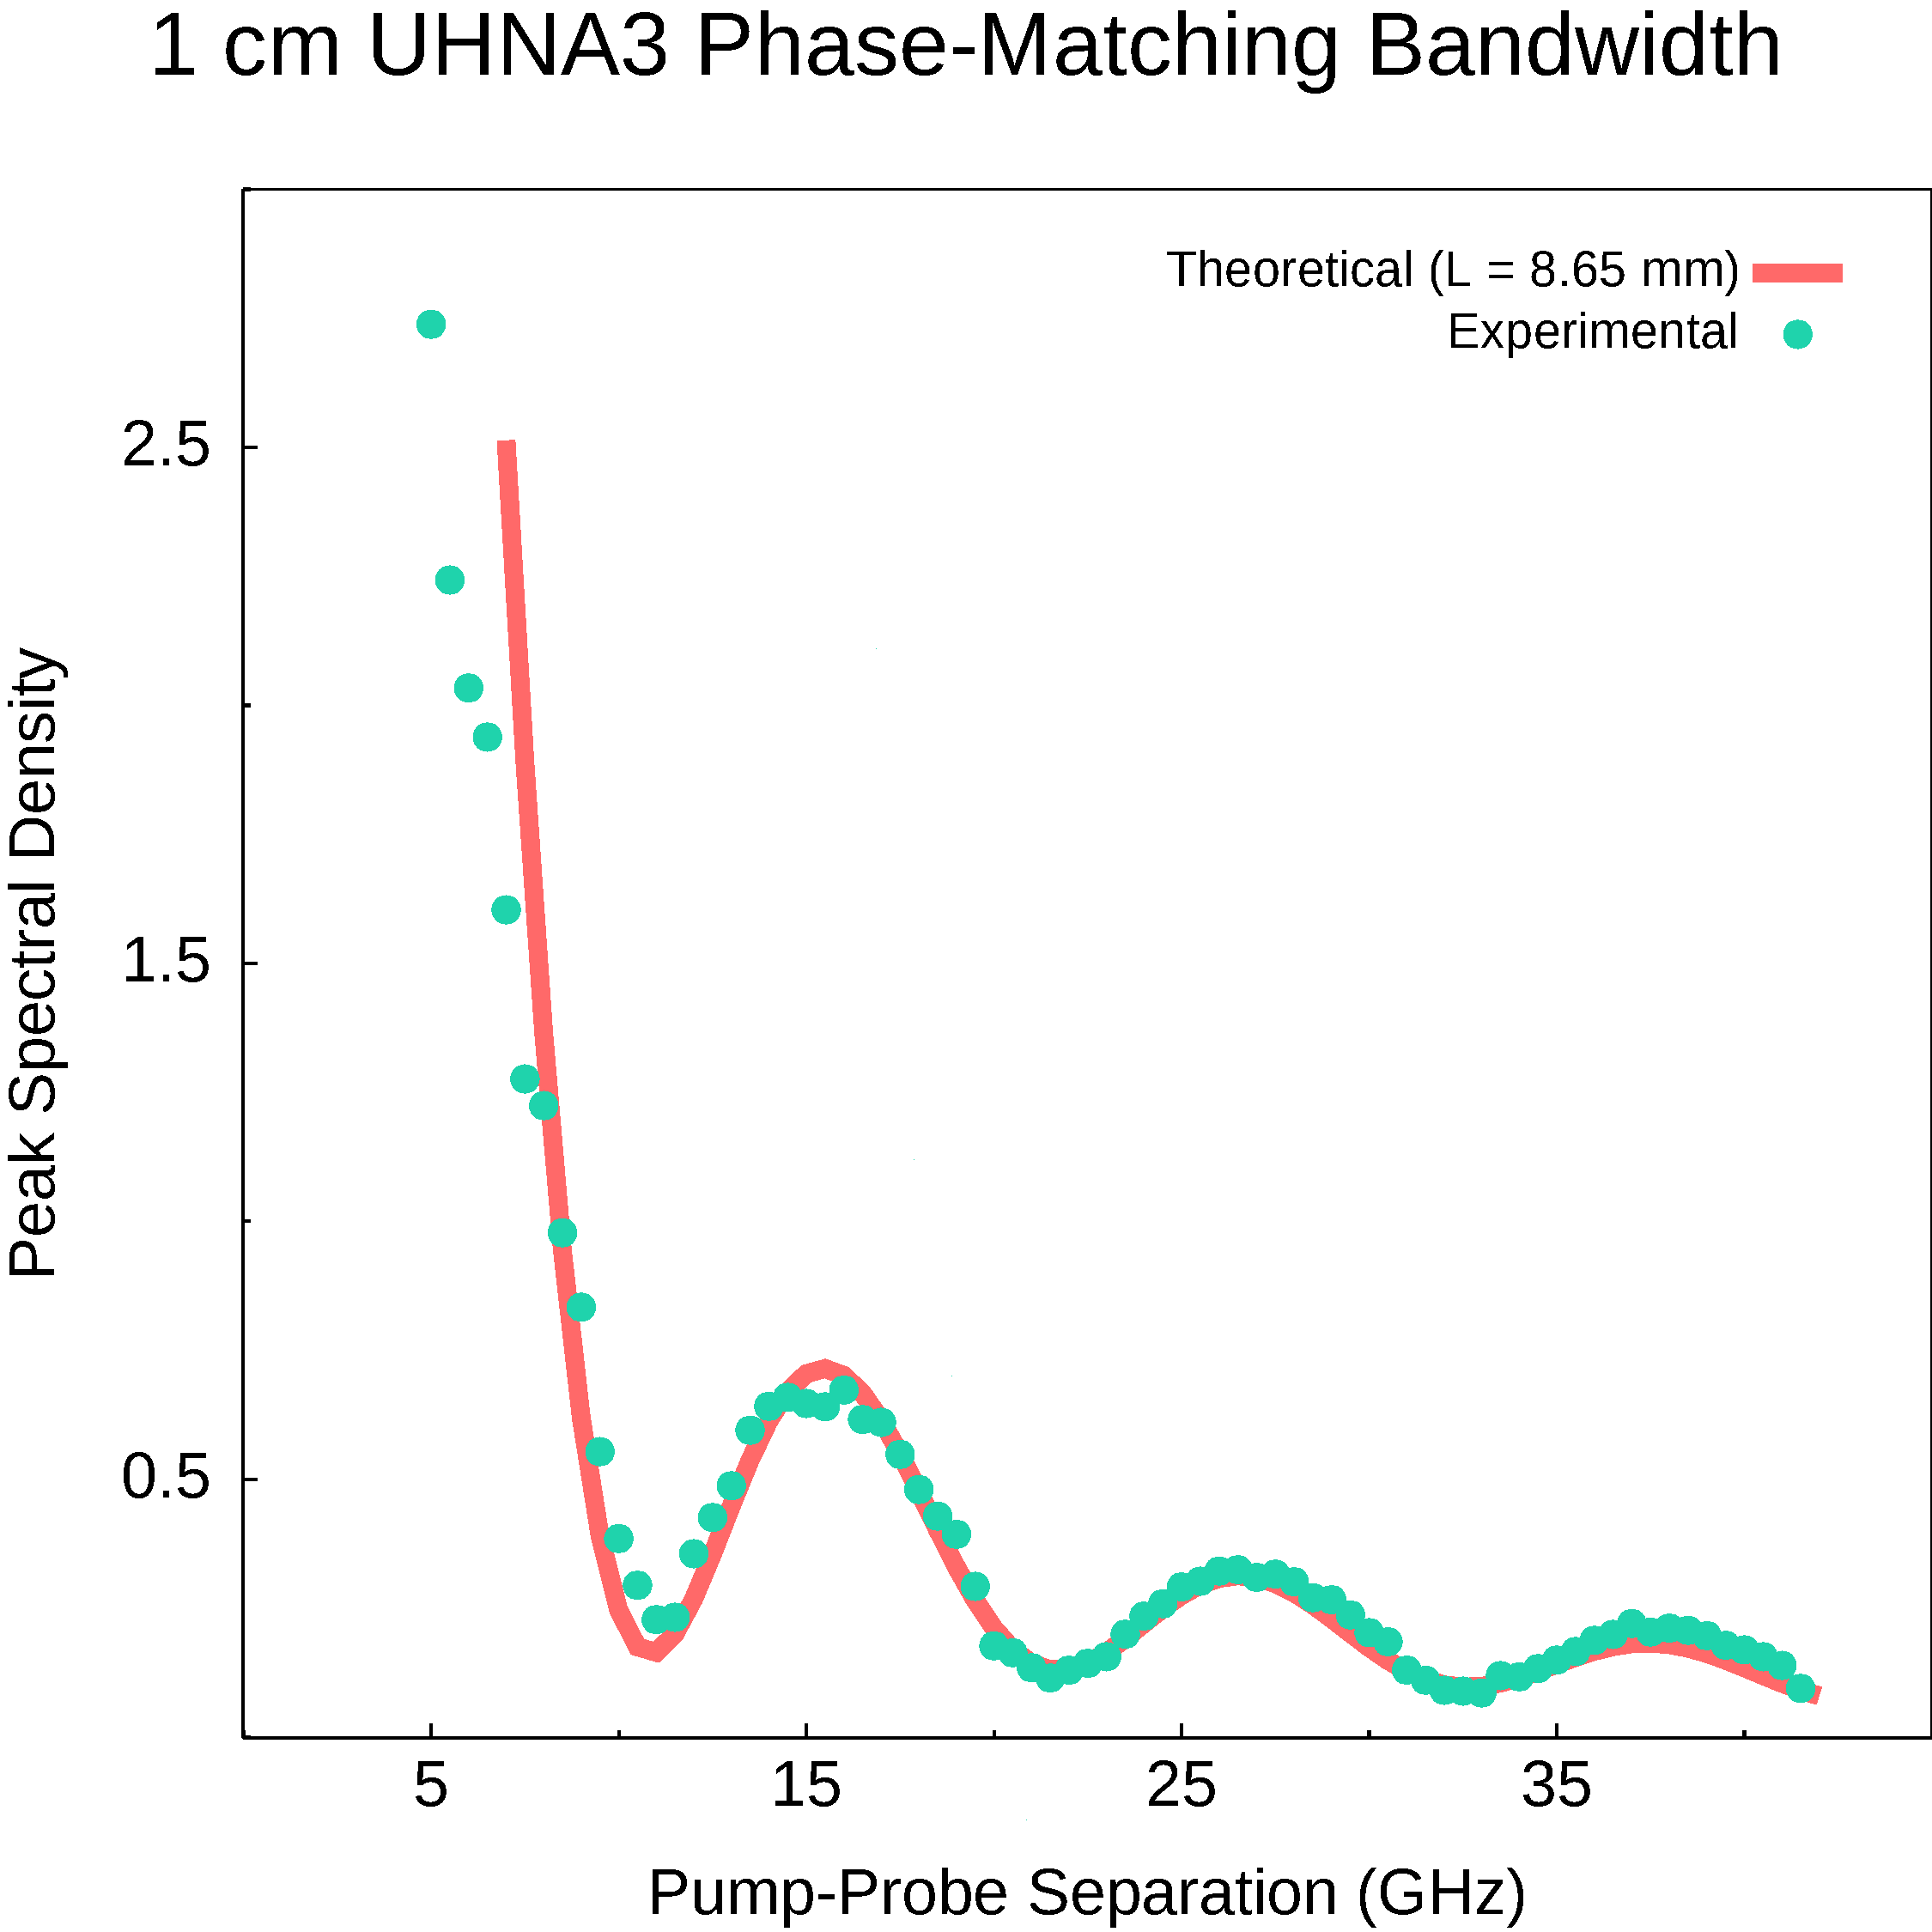
\includegraphics[width=.45\textwidth]{Phase-Match.pdf}
\caption{Phase-matching $sinc^{2}$ func}
\label{fig:Phase-Match}
\end{figure}


\section{Conclusion}
\label{Conclusion}

In conclusion, we have introduced a coherently stimulated Brillouin spectrometer utilizing a detuned pump-probe design to achieve high sensitivity and room-temperature operation in micrometer-scale samples. This approach successfully overcomes the spatial resolution limitations imposed by conventional SBS methods, demonstrating sub-10 femtowatt sensitivity in UHNA3 fiber and enabling Brillouin measurements in bulk liquid carbon disulfide with unprecedented efficiency. By relaxing phase-matching constraints, this instrument opens new possibilities for characterizing nanoscale material properties and developing nano-acousto-optic devices in standard laboratory settings without the need for cryogenic environments. Moving forward, our methodology could facilitate advancements in high-resolution phonon spectroscopy and inspire further innovations in the study of material mechanics at the microscale, reinforcing the broader applicability of Brillouin-based techniques across materials science, photonics, and sensing technologies.


\begin{acknowledgments}

\end{acknowledgments}

% Switch to appendices in one column
\clearpage % Ends the current page and all its floating elements.
\onecolumngrid % Switches to one-column format.

\begin{titlepage}
\centering
\vspace*{\stretch{1}}
{\Large Appendix:\\[10pt] A Coherently Stimulated Brillouin Spectrometer\par}
\vspace{\stretch{3}}
\end{titlepage}

\clearpage
\onecolumngrid
\clearpage

\appendix

\section{Coupled-Wave Equations}
\label{Appendix:Coupled-Wave Equations}

Here we derive the coupled wave equations that describe coherent stimulated Brillouin scattering involving a pump, Stokes, probe, and backscattered optical field given respectively by
\\
\begin{equation}
    \tilde{E}_{P}(z,t) = A_{P}e^{i(k_{P}z - \omega_{P}t)} + c.c.,
    \label{eq:Pump optical field}
\end{equation}
\\
\begin{equation}
    \tilde{E}_{S}(z,t) = A_{S}e^{i(k_{S}z - \omega_{S}t)} + c.c.,
    \label{eq:Stokes optical field}
\end{equation}
\\
\begin{equation}
    \tilde{E}_{Pr}(z,t) = A_{Pr}e^{i(k_{Pr}z - \omega_{Pr}t)} + c.c.,
    \label{eq:Probe optical field}
\end{equation}
\\
\begin{equation}
    \tilde{E}_{Sig}(z,t) = A_{Sig}e^{i(k_{Sig}z - \omega_{Sig}t)} + c.c.,
    \label{eq:Signal optical field}
\end{equation}
\\
\noindent and a common acoustic field given by
\\
\begin{equation}
    \tilde{\rho}(z,t) = \rho_{0} + \rho(z,t)e^{i(qz - \Omega t)} + c.c.,
    \label{eq:acoustic field}
\end{equation}
\\
\noindent where $\Omega = \omega_{P} - \omega_{S}$ and $q = k_{P} - k_{S} = 2k_{P}$.


\subsection{Acoustic Field}
\label{Coupled-Wave Equations:Acoustic Field}

As in the case of SBS \cite{boyd2020nonlinear}, we start by assuming that the material obeys the acoustic wave equation,
\\
\begin{equation}
    \frac{\partial^{2}\tilde{\rho}}{\partial t^{2}} - \Gamma^{\prime}\nabla^{2}\frac{\partial\tilde{\rho}}{\partial t} - v_{s}^{2}\nabla^{2}\tilde{\rho} = \nabla\cdot\vec{f},
    \label{eq:acoustic wave equation}
\end{equation}
\\
\noindent where $v_{s}$ is the sound speed in the material and $\Gamma^{\prime}$ is a damping parameter given by
\\
\begin{equation}
    \Gamma^{\prime} = \frac{1}{\rho}\left[\frac{4}{3}\eta_{s} + \eta_{b} + \frac{\kappa}{C_{p}}(\gamma - 1)\right],
\end{equation}
\\
\noindent where $\eta_{s}$ and $\eta_{b}$ are the shear and bulk viscosity coefficients of the material, respectively. The source term on the right side of Eq. (\ref{eq:acoustic wave equation}) is the divergence of the electrostrictive force:
\\
\begin{equation}
    \vec{f} = \nabla p_{st} = \nabla \cdot \Bigg[-\frac{1}{2}\epsilon_{0}\gamma_{e}\Big(\langle\tilde{E}_{P} \cdot \tilde{E}_{S}\rangle + \langle\tilde{E}_{Pr} \cdot \tilde{E}_{Sig}\rangle\Big)\Bigg],
\end{equation}
\\
which yields, after applying the slowly varying amplitude approximation,
\\
\begin{equation}
    \nabla\cdot\vec{f} = \epsilon_{0}\gamma_{e}q^{2}(A_{P}A_{S}^{*} + A_{Pr}A_{Sig}^{*})e^{i\Delta kz},
\end{equation}
\\
Where $\Delta k = (k_{Pr} - k_{Sig}) - (k_{P} - k_{S})$ is the phase mismatch between the four optical fields. Only two electrostrictive terms survive after accounting for the orthogonal polarization of the pump and Stokes fields with respect to that of the probe and backscattered signal. Inserting this electrostrictive force term and the acoustic field (Eq. (\ref{eq:acoustic field})) into Eq. (\ref{eq:acoustic wave equation}), and assuming a slowly varying acoustic amplitude, we find
\\
\begin{equation}
    -2i\Omega\frac{\partial\rho}{\partial t} - \Gamma^{\prime}2iq^{2}\Omega\rho - 2iqv_{s}^{2}\frac{\partial\rho}{\partial z} = \epsilon_{0}\gamma_{e}q^{2}(A_{P}A_{S}^{*} + A_{Pr}A_{Sig}^{*})e^{i\Delta kz},
\end{equation}
\\
which can be restated in terms of the Brillouin linewidth, $\Gamma_{B} = q^{2}\Gamma^{\prime}$, as
\\
\begin{equation}
    -2i\Omega\frac{\partial\rho}{\partial t} - 2i\Omega\Gamma_{B}\rho - 2iqv_{s}^{2}\frac{\partial\rho}{\partial z} = \epsilon_{0}\gamma_{e}q^{2}(A_{P}A_{S}^{*} + A_{Pr}A_{Sig}^{*})e^{i\Delta kz}.
    \label{eq:in terms of Brillouin linewidth}
\end{equation}
\\
Given the phonon dispersion relations $\Omega_{B} = |q_{B}|v_{s}$ and $\Omega^{2} = q^{2}\left(v^{2} - i\Omega\Gamma^{\prime}\right)$, Eq. (\ref{eq:in terms of Brillouin linewidth}) can be rewritten as
\\
\begin{equation}
    -2i\Omega\frac{\partial\rho}{\partial t} + \left(\Omega^{2} - \Omega^{2} - i\Omega\Gamma_{B}\right)\rho - 2iqv_{s}^{2}\frac{\partial\rho}{\partial z} = \epsilon_{0}\gamma_{e}q^{2}(A_{P}A_{S}^{*} + A_{Pr}A_{Sig}^{*})e^{i\Delta kz}.
    \label{eq:in terms of Omega_B}
\end{equation}
\\
We take the common assumption that the phonon propagation distance is small compared to the distance over which the source term varies significantly, which allows the spatial derivative term in Eq. (\ref{eq:in terms of Omega_B}) to be dropped. We further assume steady-state conditions such that the time derivative term also vanishes, leaving
\\
\begin{equation}
    (\Omega^{2}_{B} - \Omega^{2} - i\Omega\Gamma_{B})_{\rho} = \epsilon_{0}\gamma_{e}q^{2}(A_{P}A_{S}^{*} + A_{Pr}A_{Sig}^{*})e^{i\Delta kz}.
\end{equation}
\\
We thus find the acoustic field amplitude to be
\\
\begin{equation}
    \rho(z,t) = \epsilon_{0}\gamma_{e}q^{2}\frac{(A_{P}A_{S}^{*} + A_{Pr}A_{Sig}^{*})e^{i\Delta kz}}{\Omega_{B}^{2} - \Omega^{2} - i\Omega\Gamma_{B}}.
    \label{eq:Acoustic field amplitude}
\end{equation}


\subsection{Optical Fields}
\label{Coupled-Wave Equations:Optical Fields}

We now turn to the spatial evolution of the optical fields, described by the wave equation,
\\
\begin{equation}
    \frac{\partial^{2}\tilde{E}_{i}}{\partial z^{2}} - \frac{n^{2}}{c^{2}}\frac{\partial^{2}\tilde{E}_{i}}{\partial t^{2}} = \frac{1}{\epsilon_{0}c^{2}}\frac{\partial^{2}\tilde{P}_{i}}{\partial t^{2}},
    \label{eq:Wave equation}
\end{equation}
\\
where $i$ denotes the four optical fields, namely: pump, Stokes, probe, and the backscattered signal. The total nonlinear polarization that gives rise to the source term in the wave equation is given by
\\
\begin{equation}
    \tilde{P} = \epsilon_{0}\Delta\chi\tilde{E} = \epsilon_{0}\Delta\epsilon\tilde{E} = \epsilon_{0}\rho^{-1}\gamma_{e}\tilde{\rho}\tilde{E}.
\end{equation}
\\
The parts of $\tilde{P}$ that can act as phase-matched source terms for the optical fields are
\\
\begin{equation}
    \tilde{P}_{P} = p_{P}e^{i(k_{P}z - \omega_{P} t)} + c.c. = \frac{1}{2}\epsilon_{0}\rho_{0}^{-1}\gamma_{e}\rho A_{S}e^{i(k_{P}z - \omega_{P} t)},
    \label{eq:Pump phase-matched source term}
\end{equation}
\\
\begin{equation}
    \tilde{P}_{S} = p_{S}e^{i(-k_{S}z - \omega_{S} t)} + c.c. = \frac{1}{2}\epsilon_{0}\rho_{0}^{-1}\gamma_{e}\rho^{*} A_{P}e^{i(-k_{S}z - \omega_{S} t)},
    \label{eq:Stokes phase-matched source term}
\end{equation}
\\
\begin{equation}
    \tilde{P}_{Pr} = p_{Pr}e^{i(k_{Pr}z - \omega_{Pr} t)} + c.c. = \frac{1}{2}\epsilon_{0}\rho_{0}^{-1}\gamma_{e}\rho A_{Sig}e^{i(k_{Pr}z - \omega_{Pr} t)}e^{i\Delta kz},
    \label{eq:Probe phase-matched source term}
\end{equation}
\\
\begin{equation}
    \tilde{P}_{Sig} = p_{Sig}e^{i(-k_{Sig}z - \omega_{Sig} t)} + c.c. = \frac{1}{2}\epsilon_{0}\rho_{0}^{-1}\gamma_{e}\rho^{*} A_{Pr}e^{i(-k_{Sig}z - \omega_{Sig} t)}e^{-i\Delta kz}.
    \label{eq:Signal phase-matched source term}
\end{equation}
\\
Inserting the optical fields (Eqs. \ref{eq:Pump optical field}-\ref{eq:Signal optical field}) and phase-matched source terms (Eqs. \ref{eq:Pump phase-matched source term}-\ref{eq:Signal phase-matched source term}) into Eq. (\ref{eq:Wave equation}), we obtain
\\
\begin{equation}
    \frac{\partial A_{P}}{\partial z} + \frac{n}{c}\frac{\partial A_{P}}{\partial t} = \frac{i\omega_{P}\gamma_{e}}{2nc\rho_{0}}\rho A_{2},
\end{equation}
\\
\begin{equation}
    -\frac{\partial A_{S}}{\partial z} + \frac{n}{c}\frac{\partial A_{S}}{\partial t} = \frac{i\omega_{S}\gamma_{e}}{2nc\rho_{0}}\rho^{*}A_{P},
\end{equation}
\\
\begin{equation}
    \frac{\partial A_{Pr}}{\partial z} + \frac{n}{c}\frac{\partial A_{Pr}}{\partial t} = \frac{i\omega_{Pr}\gamma_{e}}{2nc\rho_{0}}\rho A_{Sig},
\end{equation}
\\
\begin{equation}
    -\frac{\partial A_{Sig}}{\partial z} + \frac{n}{c}\frac{\partial A_{Sig}}{\partial t} = \frac{i\omega_{Sig}\gamma_{e}}{2nc\rho_{0}}\rho^{*}A_{Pr},
\end{equation}
\\
We again assume steady-state conditions, allowing the time derivative term to be dropped. Plugging in the acoustic field amplitude (Eq. \ref{eq:Acoustic field amplitude}), we arrive at the coupled-amplitude wave equations for the optical fields,
\\
\begin{equation}
    \frac{\partial A_{P}}{\partial z} = \frac{i\epsilon_{0}\omega_{P} q^{2}\gamma_{e}^{2}}{2nc\rho_{0}}\frac{(A_{P}|A_{S}|^{2} + A_{Pr}A_{Sig}^{*}A_{S})e^{i\Delta kz}}{\Omega_{B}^{2} - \Omega^{2} - i\Omega\Gamma_{B}},
    \label{eq:Pump coupled-amplitude wave equation}
\end{equation}
\\
\begin{equation}
    \frac{\partial A_{S}}{\partial z} = -\frac{i\epsilon_{0}\omega_{S} q^{2}\gamma_{e}^{2}}{2nc\rho_{0}}\frac{(|A_{P}|^{2}A_{S}^{*} + A_{Pr}A_{Sig}^{*}A_{P})e^{-i\Delta kz}}{\Omega_{B}^{2} - \Omega^{2} + i\Omega\Gamma_{B}},
\end{equation}
\\
\begin{equation}
    \frac{\partial A_{Pr}}{\partial z} = \frac{i\epsilon_{0}\omega_{Pr} q^{2}\gamma_{e}^{2}}{2nc\rho_{0}}\frac{(A_{P}A_{S}^{*}A_{Sig} + A_{Pr}|A_{Sig}|^{2})e^{i\Delta kz}}{\Omega_{B}^{2} - \Omega^{2} - i\Omega\Gamma_{B}},
\end{equation}
\\
\begin{equation}
    \frac{\partial A_{Sig}}{\partial z} = -\frac{i\epsilon_{0}\omega_{Sig} q^{2}\gamma_{e}^{2}}{2nc\rho_{0}}\frac{(A_{P}A_{S}^{*}A_{Pr} + |A_{Pr}|^{2}A_{Sig}^{*})e^{-i\Delta kz}}{\Omega_{B}^{2} - \Omega^{2} + i\Omega\Gamma_{B}}.
    \label{eq:Signal coupled-amplitude wave equation}
\end{equation}
\\
We drop the very small signal amplitude terms on the right side of Eqs. \ref{eq:Pump coupled-amplitude wave equation}-\ref{eq:Signal coupled-amplitude wave equation} and integrate each along the effective length to get the amplitudes,
\\
\begin{equation}
  A_{P} = \frac{i\epsilon_{0}\omega_{P}q^{2}\gamma_{e}^{2}}{2nc\rho_{0}}\frac{A_{P}|A_{S}|^{2}}{\Omega_{B}^{2} - \Omega^{2} - i\Omega\Gamma_{B}} \frac{e^{i\Delta kL} - 1}{i\Delta k},
\end{equation}
\\
\begin{equation}
  A_{S} = -\frac{i\epsilon_{0}\omega_{S}q^{2}\gamma_{e}^{2}}{2nc\rho_{0}}\frac{|A_{P}|^{2}A_{S}^{*}}{\Omega_{B}^{2} - \Omega^{2} + i\Omega\Gamma_{B}} \frac{e^{-i\Delta kL} - 1}{-i\Delta k},
\end{equation}
\\
\begin{equation}
  A_{Pr} = \frac{i\epsilon_{0}\omega_{Pr}q^{2}\gamma_{e}^{2}}{2nc\rho_{0}}\frac{A_{P}A_{S}^{*}A_{Sig}}{\Omega_{B}^{2} - \Omega^{2} - i\Omega\Gamma_{B}} \frac{e^{i\Delta kL} - 1}{i\Delta k},
\end{equation}
\\
\begin{equation}
  A_{Sig} = -\frac{i\epsilon_{0}\omega_{Sig}q^{2}\gamma_{e}^{2}}{2nc\rho_{0}}\frac{A_{P}A_{S}^{*}A_{Pr}}{\Omega_{B}^{2} - \Omega^{2} + i\Omega\Gamma_{B}} \frac{e^{-i\Delta kL} - 1}{-i\Delta k}.
  \label{eq:Signal amplitude}
\end{equation}
\\
We focus on the signal amplitude given by Eq. \ref{eq:Signal amplitude}, noting that close to resonance, the denomenator of the middle term containing $\Omega$ can be approximated as,
\\
\begin{equation}
\Omega_{B}^{2} - \Omega^{2} + i\Omega\Gamma_{B} \approx \Omega_{B}(\Omega - \Omega_{B} + i\Gamma_{B}),
\end{equation}
\\
giving
\\
\begin{equation}
  A_{Sig} = -\frac{i\epsilon_{0}\omega_{Sig}q^{2}\gamma_{e}^{2}}{2nc\rho_{0}}\frac{A_{P}A_{S}^{*}A_{Pr}}{\Omega_{B}(\Omega - \Omega_{B} + i\Gamma_{B})} \frac{e^{-i\Delta kL} - 1}{-i\Delta k},
  \label{eq:resonance}
\end{equation}
\\
and in fact on resonance the expression reduces to
\\
\begin{equation}
  A_{Sig} = -\frac{i\epsilon_{0}\omega_{Sig}q^{2}\gamma_{e}^{2}}{2nc\rho_{0}}\frac{A_{P}A_{S}^{*}A_{Pr}}{\Omega_{B}i\Gamma_{B}} \frac{e^{-i\Delta kL} - 1}{-i\Delta k}.
\end{equation}
\\
Using $q = 2k_{P} = 2\omega n/c$ and $q = \Omega_{B}/v_{s}$, we can express the leading terms as
\\
\begin{equation}
  A_{Sig} = -\frac{\epsilon_{0}\omega^{2}\gamma_{e}^{2}}{c^{2}v_{s}\rho_{0}\Gamma_{B}}A_{P}A_{S}^{*}A_{Pr} \frac{e^{-i\Delta kL} - 1}{-i\Delta k},
\end{equation}
\\
where we have dropped the signal designator on $\omega$. Defining the brillouin gain factor, $g_{0}$, as Boyd does,
\\
\begin{equation}
  g_{0} = \frac{\gamma_{e}^{2}\omega^{2}}{nvc^{3}\rho_{0}\Gamma_{B}},
\end{equation}
reduces this expression to
\\
\begin{equation}
  A_{Sig} = -\epsilon_{0}ncg_{0}A_{P}A_{S}^{*}A_{Pr} \frac{e^{-i\Delta kL} - 1}{-i\Delta k}.
\end{equation}
\\
The intensity of the backscattered signal is given by the magnitude of the time-averaged Poynting vector, given by
\\
\begin{equation}
  I_{i} = 2n\epsilon_{0}c|A_{i}|^{2}, \qquad i = 1,2,3,...
\end{equation}
\\
which produces for the signal intensity
\\
\begin{equation}
  I_{Sig} = 2\epsilon_{0}nc(\epsilon_{0}ncg_{0})^{2}|A_{P}|^{2}|A_{S}^{*}|^{2}|A_{Pr}|^{2}\left|\frac{e^{-e\Delta kL} - 1}{-i\Delta k}\right|^{2}
  = 2\epsilon_{0}^{3}\epsilon_{0}n^{3}c^{3}g_{0}^{2}\frac{I_{P}}{2\epsilon_{0}nc}\frac{I_{S}}{2\epsilon_{0}nc}\frac{I_{Pr}}{2\epsilon_{0}nc}\left|\frac{e^{-e\Delta kL} - 1}{-i\Delta k}\right|^{2}.
\end{equation}
\\
The squared modulus term containing $\Delta k$ can be reduced as
\\
\begin{gather}
  \bigg|\frac{e^{-i\Delta kL} - 1}{-i\Delta k}\bigg|^{2} = \frac{(e^{-i\Delta kL} - 1)(e^{i\Delta kL} - 1)}{(\Delta k)^{2}} = \frac{L^{2}}{(\Delta kL)^{2}}\Bigg[ 2 - 2\Bigg(\frac{e^{i\Delta kL} + e^{-1\Delta kL}}{2}\Bigg)\Bigg] \notag \\ \notag \\
  = \frac{2L^{2}(1 - cos\Delta kL)}{(\Delta kL)^{2}} = \frac{4L^{2}sin^{2}\big(\frac{\Delta kL}{2}\big)}{\big(\Delta kL\big)^{2}} = \frac{L^{2}sin^{2}\big(\frac{\Delta kL}{2}\big)}{\big(\frac{\Delta kL}{2}\big)^{2}} = L^{2}sinc^{2}\bigg(\frac{\Delta kL}{2}\bigg),
\end{gather}
\\
giving as a final expression for backscattered signal intensity,
\\
\begin{equation}
I_{Sig} = \frac{1}{4}(g_{0}L)^{2}I_{P}I_{S}I_{Pr}sinc^{2}\left(\frac{\Delta kL}{2}\right).
\end{equation}
\\

% \begin{equation}
%   I_{Sig} = \frac{\epsilon_{0}^{2}\omega^{2}_{Sig}q^{4}\gamma_{e}^{4}}{4n^{2}c^{2}\rho_{0}^{2}}\frac{|A_{P}|^{2}|A_{S}^{*}|^{2}|A_{Pr}|^{2}}{\Omega_{B}^{2}\Gamma_{B}}\frac{\Gamma_{B}}{(\Omega_{B} - \Omega)^{2} + \Gamma_{B}^{2}}L^{2}sinc^{2}\left(\frac{\Delta kL}{2}\right),
% \end{equation}
% \\
% where we have multiplied top and bottom by $\Gamma_{B}$ to recognize the form of a Lorentzian. Since $\Gamma_{B}$ represents the FWHM, we modify the $\Gamma_{B}$ terms in the Lorentzian to reflect this and adopt the more physically meaningful three-parameter Lorentzian function,
% \\
% \begin{equation}
%   I_{Sig} = \frac{\epsilon_{0}^{2}\omega^{2}_{Sig}q^{4}\gamma_{e}^{4}}{4n^{2}c^{2}\rho_{0}^{2}}\frac{|A_{P}|^{2}|A_{S}^{*}|^{2}|A_{Pr}|^{2}}{\Omega_{B}^{2}\Gamma_{B}}\frac{\left(\frac{\Gamma_{B}}{2}\right)^{2}}{(\Omega_{B} - \Omega)^{2} + \left(\frac{\Gamma_{B}}{2}\right)^{2}}L^{2}sinc^{2}\left(\frac{\Delta kL}{2}\right).
% \end{equation}
% \\
% Finally, we evaluate the optical fields as
% \\
% \begin{equation}
%   I_{Sig} = \frac{\epsilon_{0}\omega^{2}_{Sig}q^{4}\gamma_{e}^{4}}{8n^{3}c^{3}\rho_{0}^{2}}\frac{I_{P}|A_{S}^{*}|^{2}|A_{Pr}|^{2}}{\Omega_{B}^{2}\Gamma_{B}}\frac{\left(\frac{\Gamma_{B}}{2}\right)^{2}}{(\Omega_{B} - \Omega)^{2} + \left(\frac{\Gamma_{B}}{2}\right)^{2}}L^{2}sinc^{2}\left(\frac{\Delta kL}{2}\right)
% \end{equation}
% \\
% \begin{equation}
%   I_{Sig} = \frac{\omega^{2}_{Sig}q^{4}\gamma_{e}^{4}}{16n^{4}c^{4}\rho_{0}^{2}}\frac{I_{P}I_{S}|A_{Pr}|^{2}}{\Omega_{B}^{2}\Gamma_{B}}\frac{\left(\frac{\Gamma_{B}}{2}\right)^{2}}{(\Omega_{B} - \Omega)^{2} + \left(\frac{\Gamma_{B}}{2}\right)^{2}}L^{2}sinc^{2}\left(\frac{\Delta kL}{2}\right)
% \end{equation}
% \\
% \begin{equation}
%   I_{Sig} = \frac{\omega^{2}_{Sig}q^{4}\gamma_{e}^{4}}{32\epsilon_{0}n^{5}c^{5}\rho_{0}^{2}}\frac{I_{P}I_{S}I_{Pr}}{\Omega_{B}^{2}\Gamma_{B}}\frac{\left(\frac{\Gamma_{B}}{2}\right)^{2}}{(\Omega_{B} - \Omega)^{2} + \left(\frac{\Gamma_{B}}{2}\right)^{2}}L^{2}sinc^{2}\left(\frac{\Delta kL}{2}\right)
% \end{equation}
% \\
% The acoustic wavevector, $q$, can be written in more convenient terms of the frequency, $\Omega$, and sound speed, $v_{s}$,
% \\
% \begin{equation}
%   I_{Sig} = \frac{\omega^{2}_{Sig}\Omega^{4}\gamma_{e}^{4}}{32\epsilon_{0}n^{5}v_{s}^{4}c^{5}\rho_{0}^{2}}\frac{I_{P}I_{S}I_{Pr}}{\Omega_{B}^{2}\Gamma_{B}}\frac{\left(\frac{\Gamma_{B}}{2}\right)^{2}}{(\Omega_{B} - \Omega)^{2} + \left(\frac{\Gamma_{B}}{2}\right)^{2}}L^{2}sinc^{2}\left(\frac{\Delta kL}{2}\right),
% \end{equation}
% \\
% and the signal frequency, $\omega_{Sig}$, can be expressed in terms of the speed of light, $c$, and the material refractive index, $n$, simplifying the expression slightly to
% \\
% \begin{equation}
%   I_{Sig} = \frac{\Omega^{4}\gamma_{e}^{4}}{32\epsilon_{0}n^{3}v_{s}^{4}c^{7}\rho_{0}^{2}}\frac{I_{P}I_{S}I_{Pr}}{\Omega_{B}^{2}\Gamma_{B}}\frac{\left(\frac{\Gamma_{B}}{2}\right)^{2}}{(\Omega_{B} - \Omega)^{2} + \left(\frac{\Gamma_{B}}{2}\right)^{2}}L^{2}sinc^{2}\left(\frac{\Delta kL}{2}\right).
% \end{equation}
% \\
% Having already made the assumption of being close to resonance ($\Omega \approx \Omega_{B}$), we allow the $\Omega$ and $\Omega_{B}$ terms to cancel, leaving
% \\
% \begin{equation}
%   I_{Sig} = \frac{\Omega^{2}\gamma_{e}^{4}}{32\epsilon_{0}n^{3}v_{s}^{4}c^{7}\rho_{0}^{2}\Gamma_{B}}I_{P}I_{S}I_{Pr}\frac{\left(\frac{\Gamma_{B}}{2}\right)^{2}}{(\Omega_{B} - \Omega)^{2} + \left(\frac{\Gamma_{B}}{2}\right)^{2}}L^{2}sinc^{2}\left(\frac{\Delta kL}{2}\right).
% \end{equation}
% \\
% We now simplify this expression as
% \\
% \begin{equation}
%   I_{Sig} = G_{CoBS}I_{P}I_{S}I_{Pr}L^{2}sinc^{2}\left(\frac{\Delta kL}{2}\right),
% \end{equation}
% \\
% where we have defined $G_{CoBS}$ to be the gain term for this 4-wave mixing coherently stimulated Brillouin scattering process,
% \\
% \begin{equation}
%   G_{CoBS} = g_{0}\frac{\left(\frac{\Gamma_{B}}{2}\right)^{2}}{(\Omega_{B} - \Omega)^{2} + \left(\frac{\Gamma_{B}}{2}\right)^{2}},
% \end{equation}
% \\
% with $g_{0}$ given by
% \\
% \begin{equation}
%   g_{0} = \frac{\Omega^{2}\gamma_{e}^{4}}{32\epsilon_{0}n^{3}v_{s}^{4}c^{7}\rho_{0}^{2}\Gamma_{B}}.
% \end{equation}
% \\

To find the power of the backscattered signal, we would integrate this intensity over the effective area. For a uniform area $A_{eff}$, this gives
\\
\begin{equation}
  P_{Sig} = I_{Sig}A_{eff} = \frac{1}{4}(g_{0}L)^{2}\frac{A_{eff}}{A_{eff}}I_{P}\frac{A_{eff}}{A_{eff}}I_{S}\frac{A_{eff}}{A_{eff}}I_{Pr}sinc^{2}\left(\frac{\Delta kL}{2}\right)A_{eff},
\end{equation}
\\
or,
\\
\begin{equation}
  P_{Sig} = \frac{1}{4}(G_{B}L)^{2}P_{P}P_{S}P_{Pr}sinc^{2}\left(\frac{\Delta kL}{2}\right),
\end{equation}
\\
where,
\\
\begin{equation}
  G_{B} = \frac{g_{0}}{A_{eff}}.
\end{equation}
\\
We can also see that off resonance, the $\Omega$ term from Eq. \ref{eq:resonance} goes to a lorentzian form after taking the squared modulus for intensity.

\newpage


\section{Scattered Power Comparison to Traditional Brillouin Scattering Processes}

This appendix provides a comparative analysis of the scattered power produced by our instrument to that of standard Brillouin scattering processes. The different behavior arises due to coherent stimulation of the acoustic mode by the pump and Stokes fields, producing a 4-wave-coupled-amplitude interaction that yields much higher scattered powers in smaller lengths than traditional Brillouin techniques. While our instrument is particularly well suited to small interaction lengths due to enhanced phase-matching relaxation, the quadradic dependence on length serves to counter-balance diminished phase-matching effects, maintaining large scattered power at larger lengths as well (greater than 1 meter). At very large lengths (greater than 1 km), the instrument is ultimately limited by the coherence length of the lasers themselves, as the process relies on the coherent stimulation of the phonon mode and thus the mutual coherence of the pump and Stokes optical fields over the full interaction length. Here we offer an exploration of the respetive performance of each technique across the entire meaningful length scale, from nanometers to kilometers.

Despite shared dependence on basic Brillouin scattering principles, the three techniques compared here (spontaneous-, stimulated-, and coherently stimulated Brillouin scattering) yield significantly different scattered power for identical experimental paramters. At small lengths, the high-gain threshold for optical stimulation of the material fluctuations is often not achievable without the use of extremely large optical powers. This prevents the system from entering a process of exponential growth of the scattered Stokes light indicative of stimulated Brillouin scattering.\cite{boyd2020nonlinear} In this low-gain regime, any scattered Stokes light is spontanously scattered from thermal fluctuations of the material, or from quantum-mechanical fluctuations of materials at the ground state. The low-gain regime is defined by an overall process gain factor, denoted by $G = G_{P}P_{P}L$, which is much less than unity ($G \ll 1$). Here, $G_{B}$ is the effective Brillouin gain in $W^{-1}m^{-1}$ ($G_{B} = \frac{g}{A_{eff}}$), $P_{P}$ is the pump power, and $L$ is the effective length. This spontaneous scattering process follows a linear growth trend described by Boyd et al in 1990\cite{boyd1990noise} as

\begin{equation}
  R = \frac{\langle|E_{S}|^{2}\rangle}{\langle|E_{P}|^{2}\rangle} = (\bar{n} + 1)g\hbar\omega_{S}\Gamma_{B}\frac{L}{4A_{eff}},
\end{equation}

where R is the reflectivity, or the ratio of scattered Stokes intensity to incident pump intensity, and $\bar{n} = (e^{\frac{\hbar\Omega_{B}}{k_{b}T}} - 1)^{-1}$ is the mean number of phonons occupying the mode due to thermal fluctuations of the material. Rearranging this equation and converting to effective Brillouin gain, $G_{B}$, and power by applying the effective area, we arrive at the scattered power of the Stokes spontaneous Brillouin scattering process,

\begin{equation}
  P_S = \frac{1}{4}G_{B}P_{P}L\hbar\omega_{S}\Gamma_{B}(\bar{n} + 1).
  \label{eq:SponBSnbar}
\end{equation}

At room temperature and typical Brillouin frequencies in the GHz range, the quantity $k_{b}T \gg \hbar\Omega_{B}$, allowing

\begin{equation}
e^{\frac{\hbar\Omega_{B}}{k_{b}T}} \approx 1 + \frac{\hbar\Omega_{B}}{k_{b}T}
\end{equation}

to be a good approximation. We thus find that

\begin{equation}
(\bar{n} + 1) \approx \bar{n} \approx \frac{k_{b}T}{\hbar\Omega_{B}}.
\end{equation}

Inserting this reduced quantity into Eq. \ref{eq:SponBSnbar}, we arrive at a convenient expression for the scattered power of the Stokes spontaneous Brillouin scattering process,

\begin{equation}
  P_{S, \,\textit{SponBS}} = \frac{G_{B}P_{P}L\omega_{S}\Gamma_{B}k_{b}T}{4\Omega_{B}}.
\end{equation}

It may be noted that this is equivalent to the expression for the \textit{forward} Stokes spontaneous Brillouin scattering process derived by Kharel et al in 2016.\cite{kharel2016noise} While each describe seemingly distinct processes, the underlying physics of light coupling to acoustic waves is shared and leads to identical scaling laws for scattered power in the low-gain (spontaneous) regime.

Next we turn to the high-gain regime leading to a stimulated Brillouin scattering process. This regime is defined by an overall process gain factor, $G = G_{P}P_{P}L$, that is much greater than unity ($G \gg 1$). For organic liquids, this crossover threshold from spontaneous to stimulated regimes occurs in the range of $20 < G < 25,$\cite{boyd1990noise} whereas for typical lengths of single mode fiber it can be lower\cite{ippen1972stimulated} owing to the small effective area compared to longer effective lengths of fiber typically used.

The reflectivity of a stimulated Brillouin scattering process in the high-gain regime is given by \cite{boyd1990noise}

\begin{equation}
  R = \frac{\langle|E_{S}|^{2}\rangle}{\langle|E_{P}|^{2}\rangle} = \frac{Y}{\sqrt{\pi}}\frac{e^{G}}{G^{\frac{3}{2}}},
\end{equation}

where $Y$ is the reflectivity of the low-gain (spontaneous) regime given above and $G$ is the overall process gain factor, $G = G_{P}P_{P}L$. Again, converting to the effective Brillouin gain, $G_{B}$, and power by applying the effective area, we solve for the scattered power of the Stokes field,

\begin{equation}
  P_{S, \,\textit{StimBS}} = \frac{G_{B}P_{P}L\omega_{S}\Gamma_{B}k_{b}T}{4\sqrt{\pi}\Omega_{B}}\frac{e^{G}}{G^{\frac{3}{2}}}
  \label{StimBSUndepletedPump}
\end{equation}

This expression captures the exponential growth in scattered power as any parameter within the overall process gain factor, $G = G_{B}P_{P}L$, increases. However, this exponential growth can only continue while the pump is not significantly undepleted. Once the scattered power described by Eq. \ref{eq:StimBSUndepletedPump} grows to become a significant portion of the driving pump power, the exponential increase in scattered Stokes power turns to an asymptotic approach of the pump power. For very large $G$, virtually all of the pump energy is converted to scattered Stokes energy in a complete transfer process.\cite{boyd2020nonlinear} To account for pump depletion, we numerically solve the transendental equation derived in Boyd's Nonlinear Optics which describes the effects of pump depletion, given here in terms of power,

\begin{equation}
  P_S(L) = \frac{P_S(0)x(1 - x)}{e^{G_{B}P_{P}(0)L(1 - x)} - x},
\end{equation}

where $x = P_S(0)/P_P(0)$, or the ratio of the unknown Stokes power at the end of its journey ($z=0$) to the known pump power at the beginning (also $z=0$). This solution for $x$, for given system parameters such as length, offers via its definition the solution to the unknown power of the scattered Stokes light at the end of its traversal through the effective length (corresponding to $z=0$ since it propagates opposite to the pump),

\begin{equation}
  P_S(0) = xP_{P}(0).
\end{equation}

This numeric solution to the scattered power in the high-gain (stimulated) Brillouin scattering regime with pump depletion effects at large $G$ is plotted for varying effective lengths in Fig. \ref{fig:SponBSvsStimBSvsCoBS}, along with the analytical solutions derived previously for the low-gain (spontaneous) regime and our coherently stimulated Brillouin spectrometer given by Eq. \ref{Eq:Theoretical Framework:Scattered Power}. Relevant parameters used across all three processes are given in Tables \ref{tab:CoBS Parameters} and \ref{tab:SBS Parameters}.


% Here, we clarify why SBS, typically a strong scattering mechanism, produces minimal scattered power in short fiber lengths, whereas our instrument can yield much higher powers under similar conditions. Theoretical insights and numerical examples with specific parameters for germania-doped UHNA3 fiber are provided to illustrate this difference.
%
% SBS is a nonlinear optical process where an intense pump laser beam interacts with thermally excited acoustic phonons in the fiber, leading to the generation and amplification of a backward-propagating Stokes wave. This interaction satisfies energy and momentum conservation:
%
% \begin{equation}
% \omega_{P} = \omega_{S} + \Omega, \quad \mathbf{k}_{P} = \mathbf{k}_{S} + \mathbf{q},
% \end{equation}
%
% where $\omega_{P}$, $\omega_{S}$, and $\Omega$ are the angular frequencies of the pump and Stokes waves, $\Omega$ is the angular frequency of the acoustic phonon, and $\mathbf{k}_{P}$, $\mathbf{k}_{S}$, and $\mathbf{q}$ are the corresponding wavevectors. In SBS, the initial Stokes wave originates from spontaneous Brillouin scattering due to thermal fluctuations within the medium. This initial Stokes power, $P_{S}(0)$, is extremely low—typically on the order of picowatts (pW) or femtowatts (fW). The Stokes wave can be amplified through its interaction with the pump beam over the fiber length, governed by the coupled-wave equations. Under the assumption of negligible pump depletion (valid in the low-gain regime), the Stokes power at the end of the length of media ($z = L$) is
%
% \begin{equation}
% P_{S}(L) = P_{S}(0) e^{G_{B} P_{P} L},
% \end{equation}
%
% where is the effective Brillouin gain given by Equation \ref{Eq:Effective Brillouin Gain}, $P_{P}$ the pump power, and $L$ the fiber length. In the low-gain regime ($G_{B} P_{P} L \ll 1$), the exponential can be approximated with a series expansion by $e^{G_{B}P_{P}L} \approx 1 + G_{B}P_{P}L$, making the increase in Stokes power
%
% \begin{equation}
% \Delta P_S = P_S(L) - P_S(0) \approx P_S(0) G_{B}P_{P}L.
% \end{equation}
%
% A critical factor limiting SBS in the low-gain regime is phonon dissipation. Acoustic phonons have a finite lifetime ($\tau$) due to material absorption and scattering processes. This finite lifetime introduces a dissipation rate ($\Gamma = 1/\tau$) that counteracts the amplification process. The effective Brillouin gain $G_{B}$ is inversely proportional to this phonon dissipation rate, or Brillouin linewidth, ($\Gamma_{B}$), which is related to the phonon lifetime, given by
%
% \begin{equation}
% G_{B} \propto \frac{1}{\Gamma_{B}} = \tau.
% \end{equation}
%
% High phonon dissipation (short $\tau$) reduces $G_{B}$, thus limiting Stokes amplification, which scales by $G_{B}P_{P}L$. In short media, the limited interaction length further restricts significant amplification of the Stokes wave. For SBS to achieve significant amplification, $G_{B}P_{P}L$ must be large enough to induce exponential growth of the Stokes wave. In long fibers with sufficient pump power, the Stokes power can increase exponentially due to the positive feedback loop between the pump, Stokes, and acoustic phonons. However, in short fibers like our 1 cm UHNA3 fiber, $G_{B}P_{P}L$ remains small, placing the system in the low-gain regime. In this regime, the Stokes power increases only linearly with distance, and the amplification is insufficient to produce a detectable scattered signal. The phonon dissipation within the material limits the build-up of the phonon population over time, causing acoustic phonons to decay before they can significantly contribute to Stokes wave amplification and preventing the system from reaching the high-gain regime.
%
% Our coherently stimulated Brillouin spectrometer, in contrast, utilizes strong pump, Stokes, and probe waves that are supplied externally. Unlike SBS, where the Stokes wave originates from thermal noise, our instrument supplies all interacting waves externally, with significant input powers, and hence does not rely on spontaneous scattering to initiate the interaction. Instead, it benefits from coherent interactions among the input optical waves and the acoustic phonons, leading to efficient energy transfer. As seen in Equation \ref{Eq:Theoretical Framework:Scattered Power}, the scattered power depends on $(G_{B} L)^{2}$ and the product of the input powers, allowing for substantial scattered signals even in short fibers.

\begin{figure}[t]
\centering
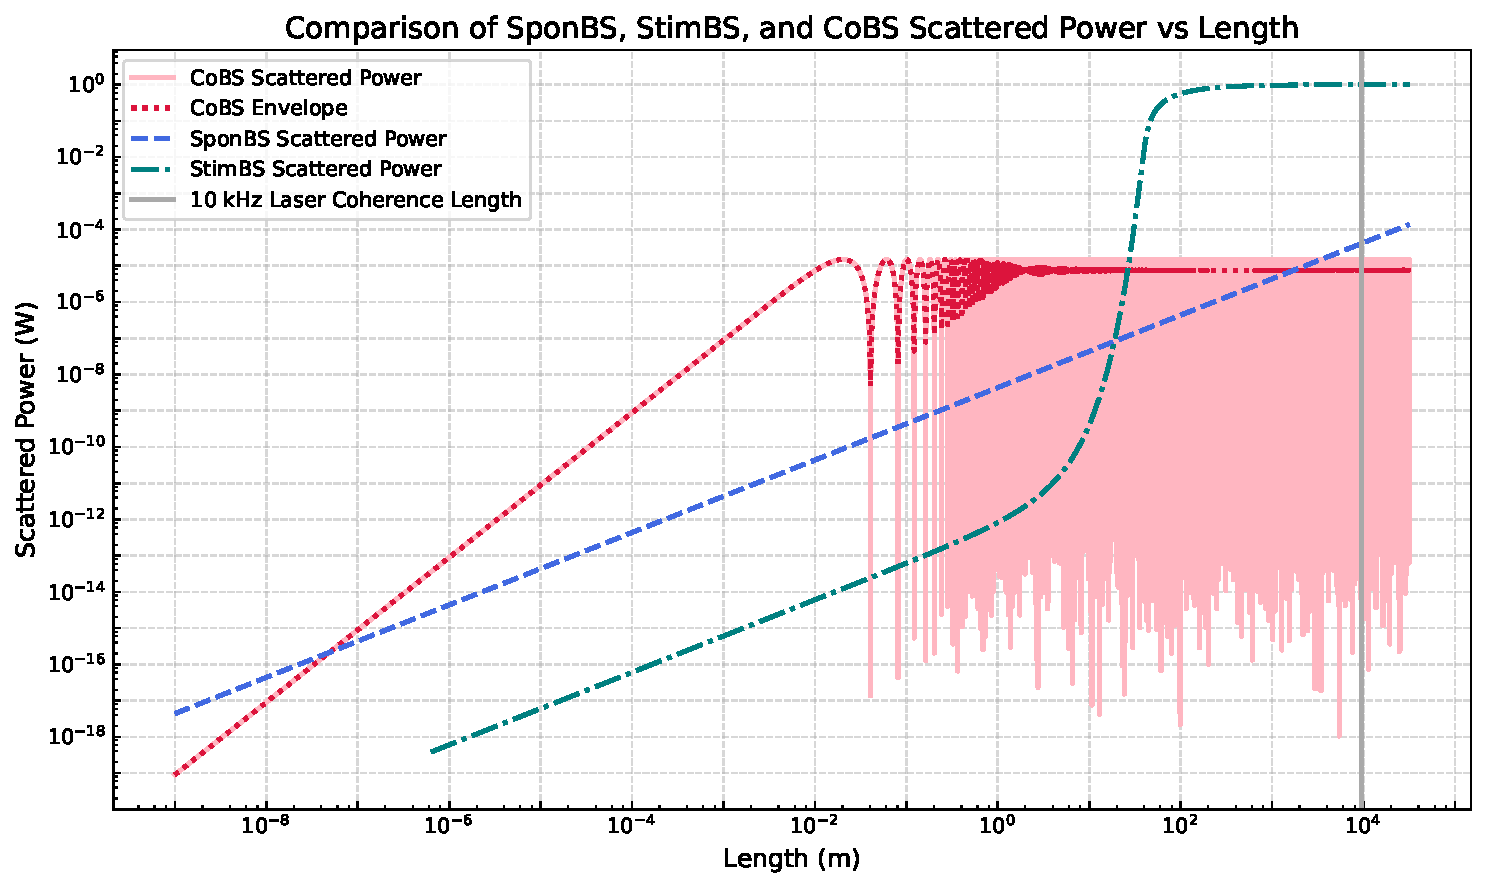
\includegraphics[width=.95\textwidth]{SponBSvsStimBSvsCoBS.pdf}
\caption{Comparison of scattered power from a spontaneous Brillouin scattering process and our coherently stimulated Brillouin spectrometer.}
\label{fig:SponBSvsStimBSvsCoBS}
\end{figure}

To quantify the difference, we consider typical measurement parameters, given in Table \ref{tab:SBS Comparison Parameters}, applied to a 1 cm length of UHNA3 fiber.

\begin{table}[h]
  \centering
  \textbf{Coherently Stimulated Brillouin Scattering Process Model System Parameters}
  \renewcommand{\arraystretch}{1.2}
  \begin{tabular}{|c|c|c|c|c|}
    \hline
    $G_{B}$ & $P_{P}$ & $P_{S}$ & $P_{Pr}$ & $\Delta\lambda$ \\
    \hline
    0.6 $W^{-1} m^{-1}$ & 1 $W$ & 1 $W$ & 1 $W$ & 20 pm \\
    \hline
  \end{tabular}
  \caption{Parameters relevant to the coherently stimulated backward Brillouin scattering process for the example UHNA3 fiber. $G_{B}$ is the effective Brillouin gain, $P_{P}$ is the pump power, $P_{S}$ is the Stokes power, $P_{Pr}$ is the probe power, and $\Delta\lambda$ is the wavelength detuning of the probe from the pump.}
  \label{tab:CoBS Parameters}
\end{table}

\begin{table}[h]
  \centering
  \textbf{Spontaneous and Stimulated Scattering Process Model System Parameters}
  \renewcommand{\arraystretch}{1.2}
  \begin{tabular}{|c|c|c|c|c|c|c|c|c|}
    \hline
    $G_{B}$ & $P_{P}$ & $P_{S,seed}$ & $n$ & $\lambda_P$ & $\Gamma_{B}$ & $k_{B}$ & $T$ & $\Omega_{B}$ \\
    \hline
    0.6 $W^{-1} m^{-1}$ & 1 $W$ & $1$ pW & 1.48 & $1549$ nm & $2\pi \cdot 80$ MHz & $1.38 \times 10^{-23}$ J/K & 295 K & $2\pi \cdot 9.18$ GHz \\
    \hline
  \end{tabular}
  \caption{Parameters relevant to the spontaneous and/or stimulated backward Brillouin scattering processes for the example UHNA3 fiber. $G_{B}$ is the Brillouin gain coefficient, $P_{P}$ is the pump power, $\omega$ is the optical angular frequency, $\Gamma_{B}$ is the acoustic damping rate, $k_{B}$ is Boltzmann's constant, $T$ is the temperature, and $\Omega_{B}$ is the acoustic angular frequency.}
  \label{tab:SBS Parameters}
\end{table}


% The amplification scaling term ($G_{B}P_{P}L$) for SBS is only 0.003 in this case, which is much less than 1, placing the SBS process under these conditions in the low-gain regime with minimal amplification. The increase in Stokes power ($\Delta P_{S}$) is given by,
%
% \begin{equation}
% \Delta P_{S} = P_{S}(0)G_{B}P_{P}L = 3 \times 10^{-15}\, \, W = 3 \, fW.
% \end{equation}
%
% This result indicates that the scattered power from SBS is approximately $3 \, fW$, which is too low to be detected with standard photodetectors.
%
% The scattered signal power ($P_{Sig}$) of our instrument is calculated using Equation \ref{Eq:Theoretical Framework:Scattered Power} with the parameters listed in Table \ref{tab:SBS Comparison Parameters},
%
% \begin{equation}
% P_{Sig} = \frac{1}{4}\left(G_{B}L\right)^{2}P_{P}P_{S}P_{Pr}\text{sinc}^{2}\left(\frac{\Delta k L}{2}\right) = 1.07\times10^{-6} \, W = 1.07 \, \mu W.
% \end{equation}
%
% %Kharel2016 SponBS: equation 49: 21.9 pW
%
% The scattered power produced by our instrument is approximately $1.07 \, \mu W$, which is readily detectable with standard photodetectors. This comparison demonstrates that, under identical experimental conditions, our instrument produces a significantly higher scattered power than SBS in a short fiber length. This is because SBS relies on amplifying a weak initial Stokes wave over a short interaction length, but the low gain parameter and phonon dissipation prevent significant amplification, resulting in an undetectable scattered power. Our technique, however, utilizes strong input waves and coherent interactions, leading to a measurable scattered signal even in short length media. Therefore, our instrument offers a significant advantage over SBS for generating detectable scattered signals with low Brillouin gain or small interaction length.

\newpage

\section{Pump, Stokes, and Probe Contribute Equally}

Equation \ref{Eq:Theoretical Framework:Scattered Power} gives the somewhat unintuitive result that the powers of the Pump, Stokes, and Probe waves contribute equally to the resulting scattered power of the Signal and invites verification with a miniexperiment. Initially, this experiment was motivated by a practical consideration: determination of whether the placement of a high power amplifier on any specific line of the setup (Pump, Stokes, or Probe) would offer any advantage over another.

To test this, we conducted a controlled experiment with a 1 mm carbon disulfide ($CS_{2}$) sample. For each measurement, one of the three source powers (Pump, Stokes, or Probe) was systematically reduced by 75\% while holding the others constant and ensuring consistent experimental conditions across trials. Table \ref{tab:PSPr-Contribute-Equally} shows the respective powers for each source during the three measurements, along with the multiplicative total contribution of the three powers for each measurement towards the generation of scattered power of the Signal.

\begin{table}[h]
  \centering
  \renewcommand{\arraystretch}{1.2}
  \begin{tabular}{|c|c|c|c|c|}
    \hline
    \textbf{Measurement} & \textbf{Pump Power (mW)} & \textbf{Stokes Power (mW)} & \textbf{Probe Power (mW)} & \textbf{Total (mW$^{3}$)} \\
    \hline
    Pump Lower & 19.190 & 32.210 & 54.560 & 3.372 $\times 10^{4}$ \\
    Stokes Lower & 76.600 & 8.020 & 54.650 & 3.359 $\times 10^{4}$ \\
    Probe Lower & 76.600 & 32.530 & 13.480 & 3.359 $\times 10^{4}$ \\
    \hline
  \end{tabular}
    \caption{Power values for each source (Pump, Stokes, Probe) across the three measurements, with the multiplicative total power for each setup.}
    \label{tab:PSPr-Contribute-Equally}
\end{table}

Figure \ref{fig:PSPr-Contribute-Equally} displays the average results from these three measurements, plotted with error bars representing one standard deviation of the mean. For increased certainty, Figure \ref{fig:PSPr-Contribute-Equally-2sigma} presents the same data with error bars extended to two standard deviations, providing additional confidence in the reproducibility of the results. This experiment confirms that the scattered Signal power indeed depends equally on each of the three contributing wave powers, as expected from the theoretical framework. Consequently, boosting the power of any of the three sources affects the Signal power equally, allowing flexibility in pragmatic design across any of the three lines. Ultimately, this result reinforces the reliability of Equation \ref{Eq:Theoretical Framework:Scattered Power} for predicting Signal power across a range of power distributions within practical settings.

% \begin{figure}[h]
%   \centering
%   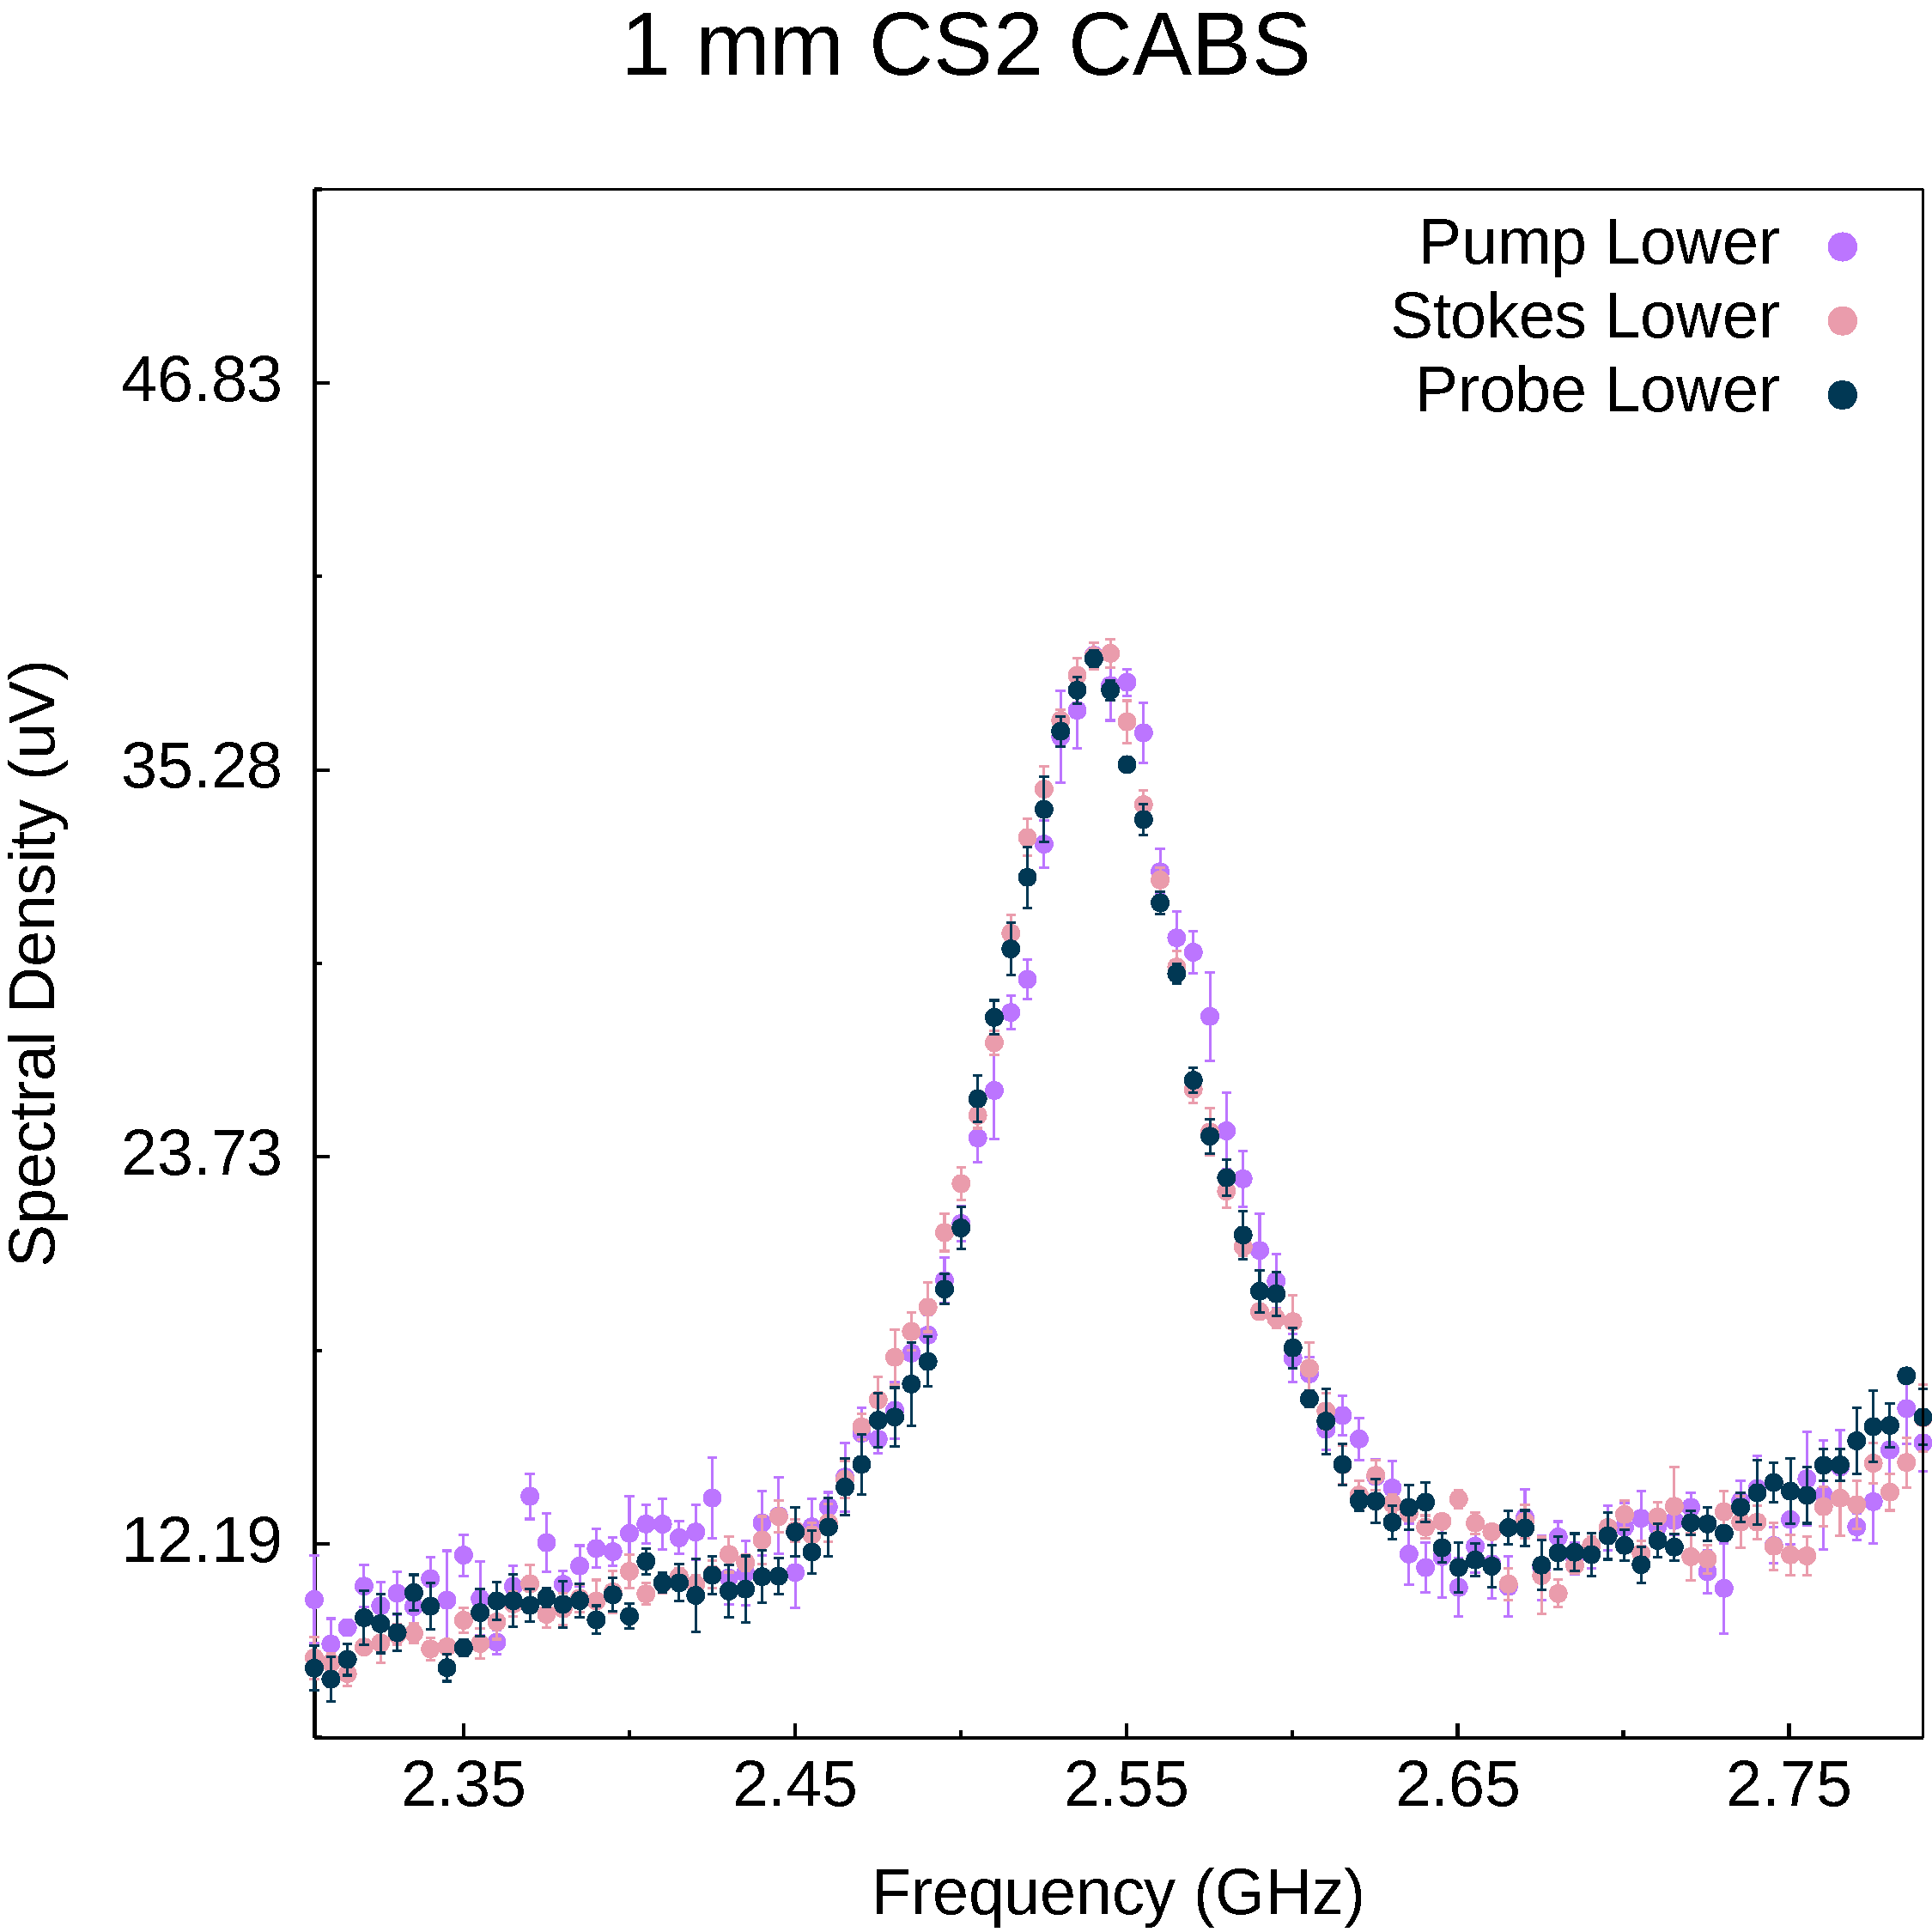
\includegraphics[width=.45\textwidth]{PSPr-Contribute-Equally.pdf}
%   \caption{Signal power contributions with error bars representing one standard deviation of the mean for each measurement.}
%   \label{fig:PSPr-Contribute-Equally}
% \end{figure}
%
% \begin{figure}[h]
%   \centering
%   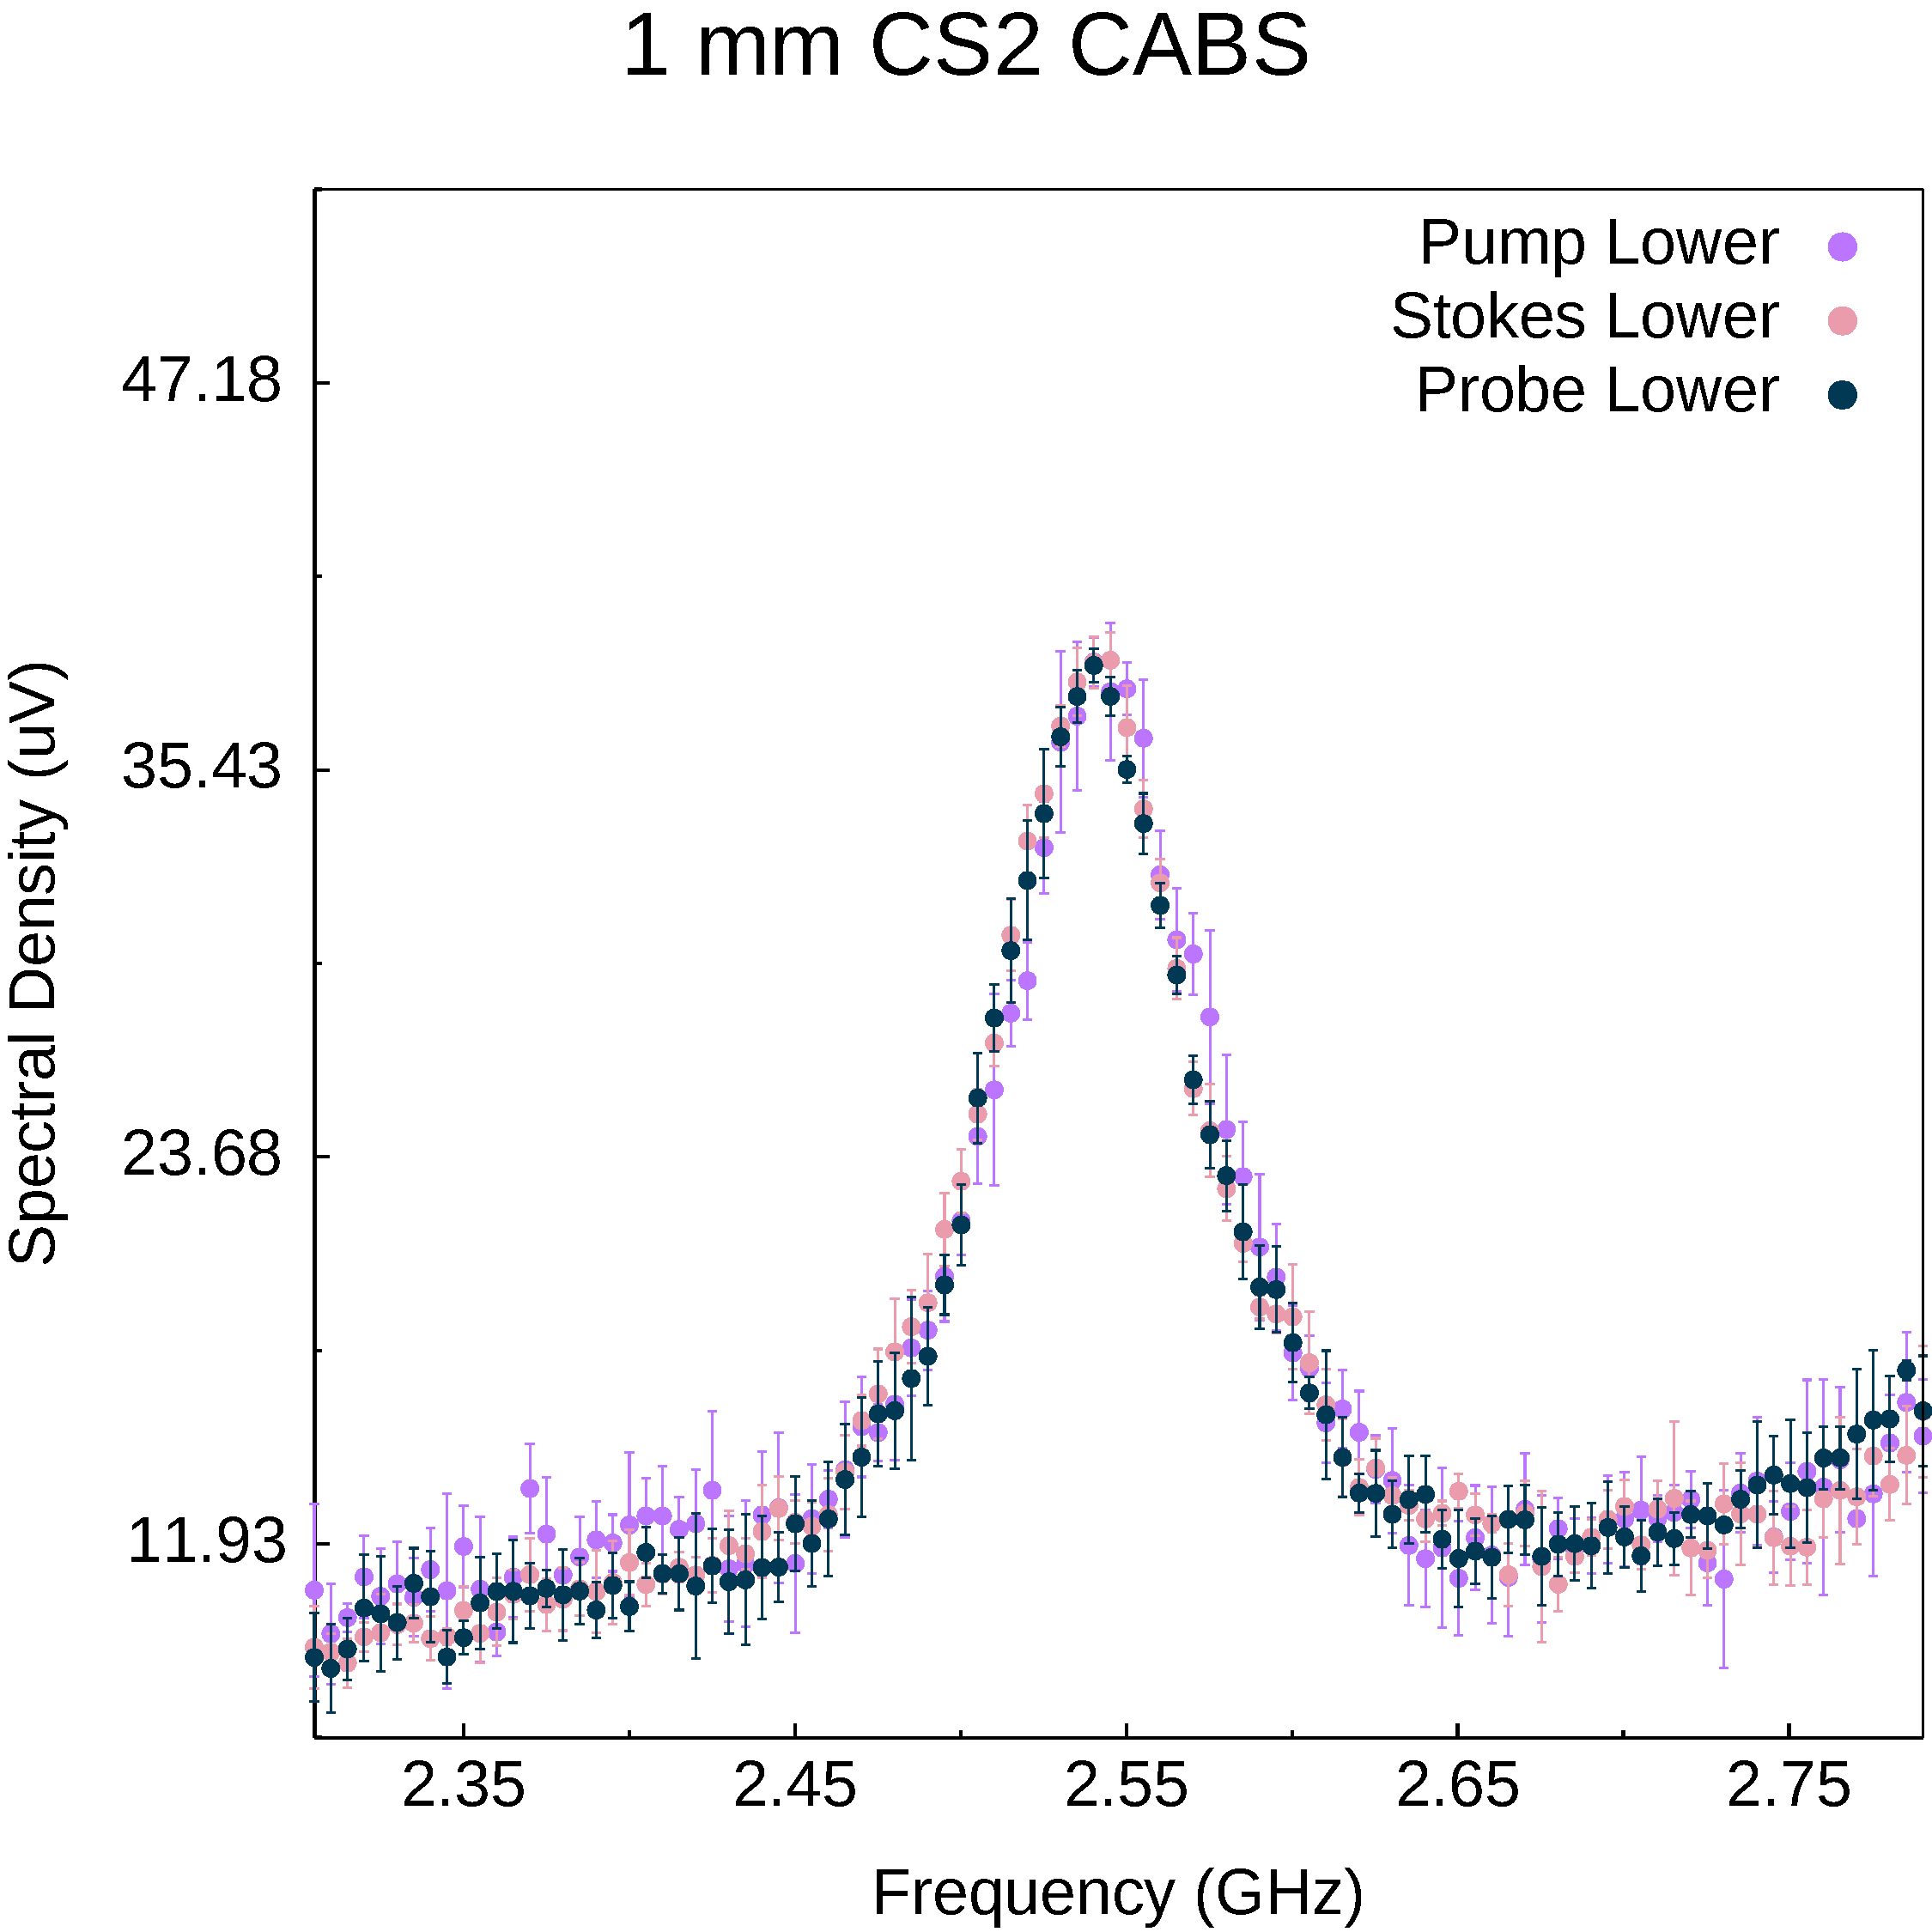
\includegraphics[width=.45\textwidth]{PSPr-Contribute-Equally-2sigma.pdf}
%   \caption{Signal power contributions with error bars extended to two standard deviations of the mean for each measurement.}
%   \label{fig:PSPr-Contribute-Equally-2sigma}
% \end{figure}

\begin{figure}[h]
  \centering
  \begin{subfigure}{0.45\textwidth}
    \centering
    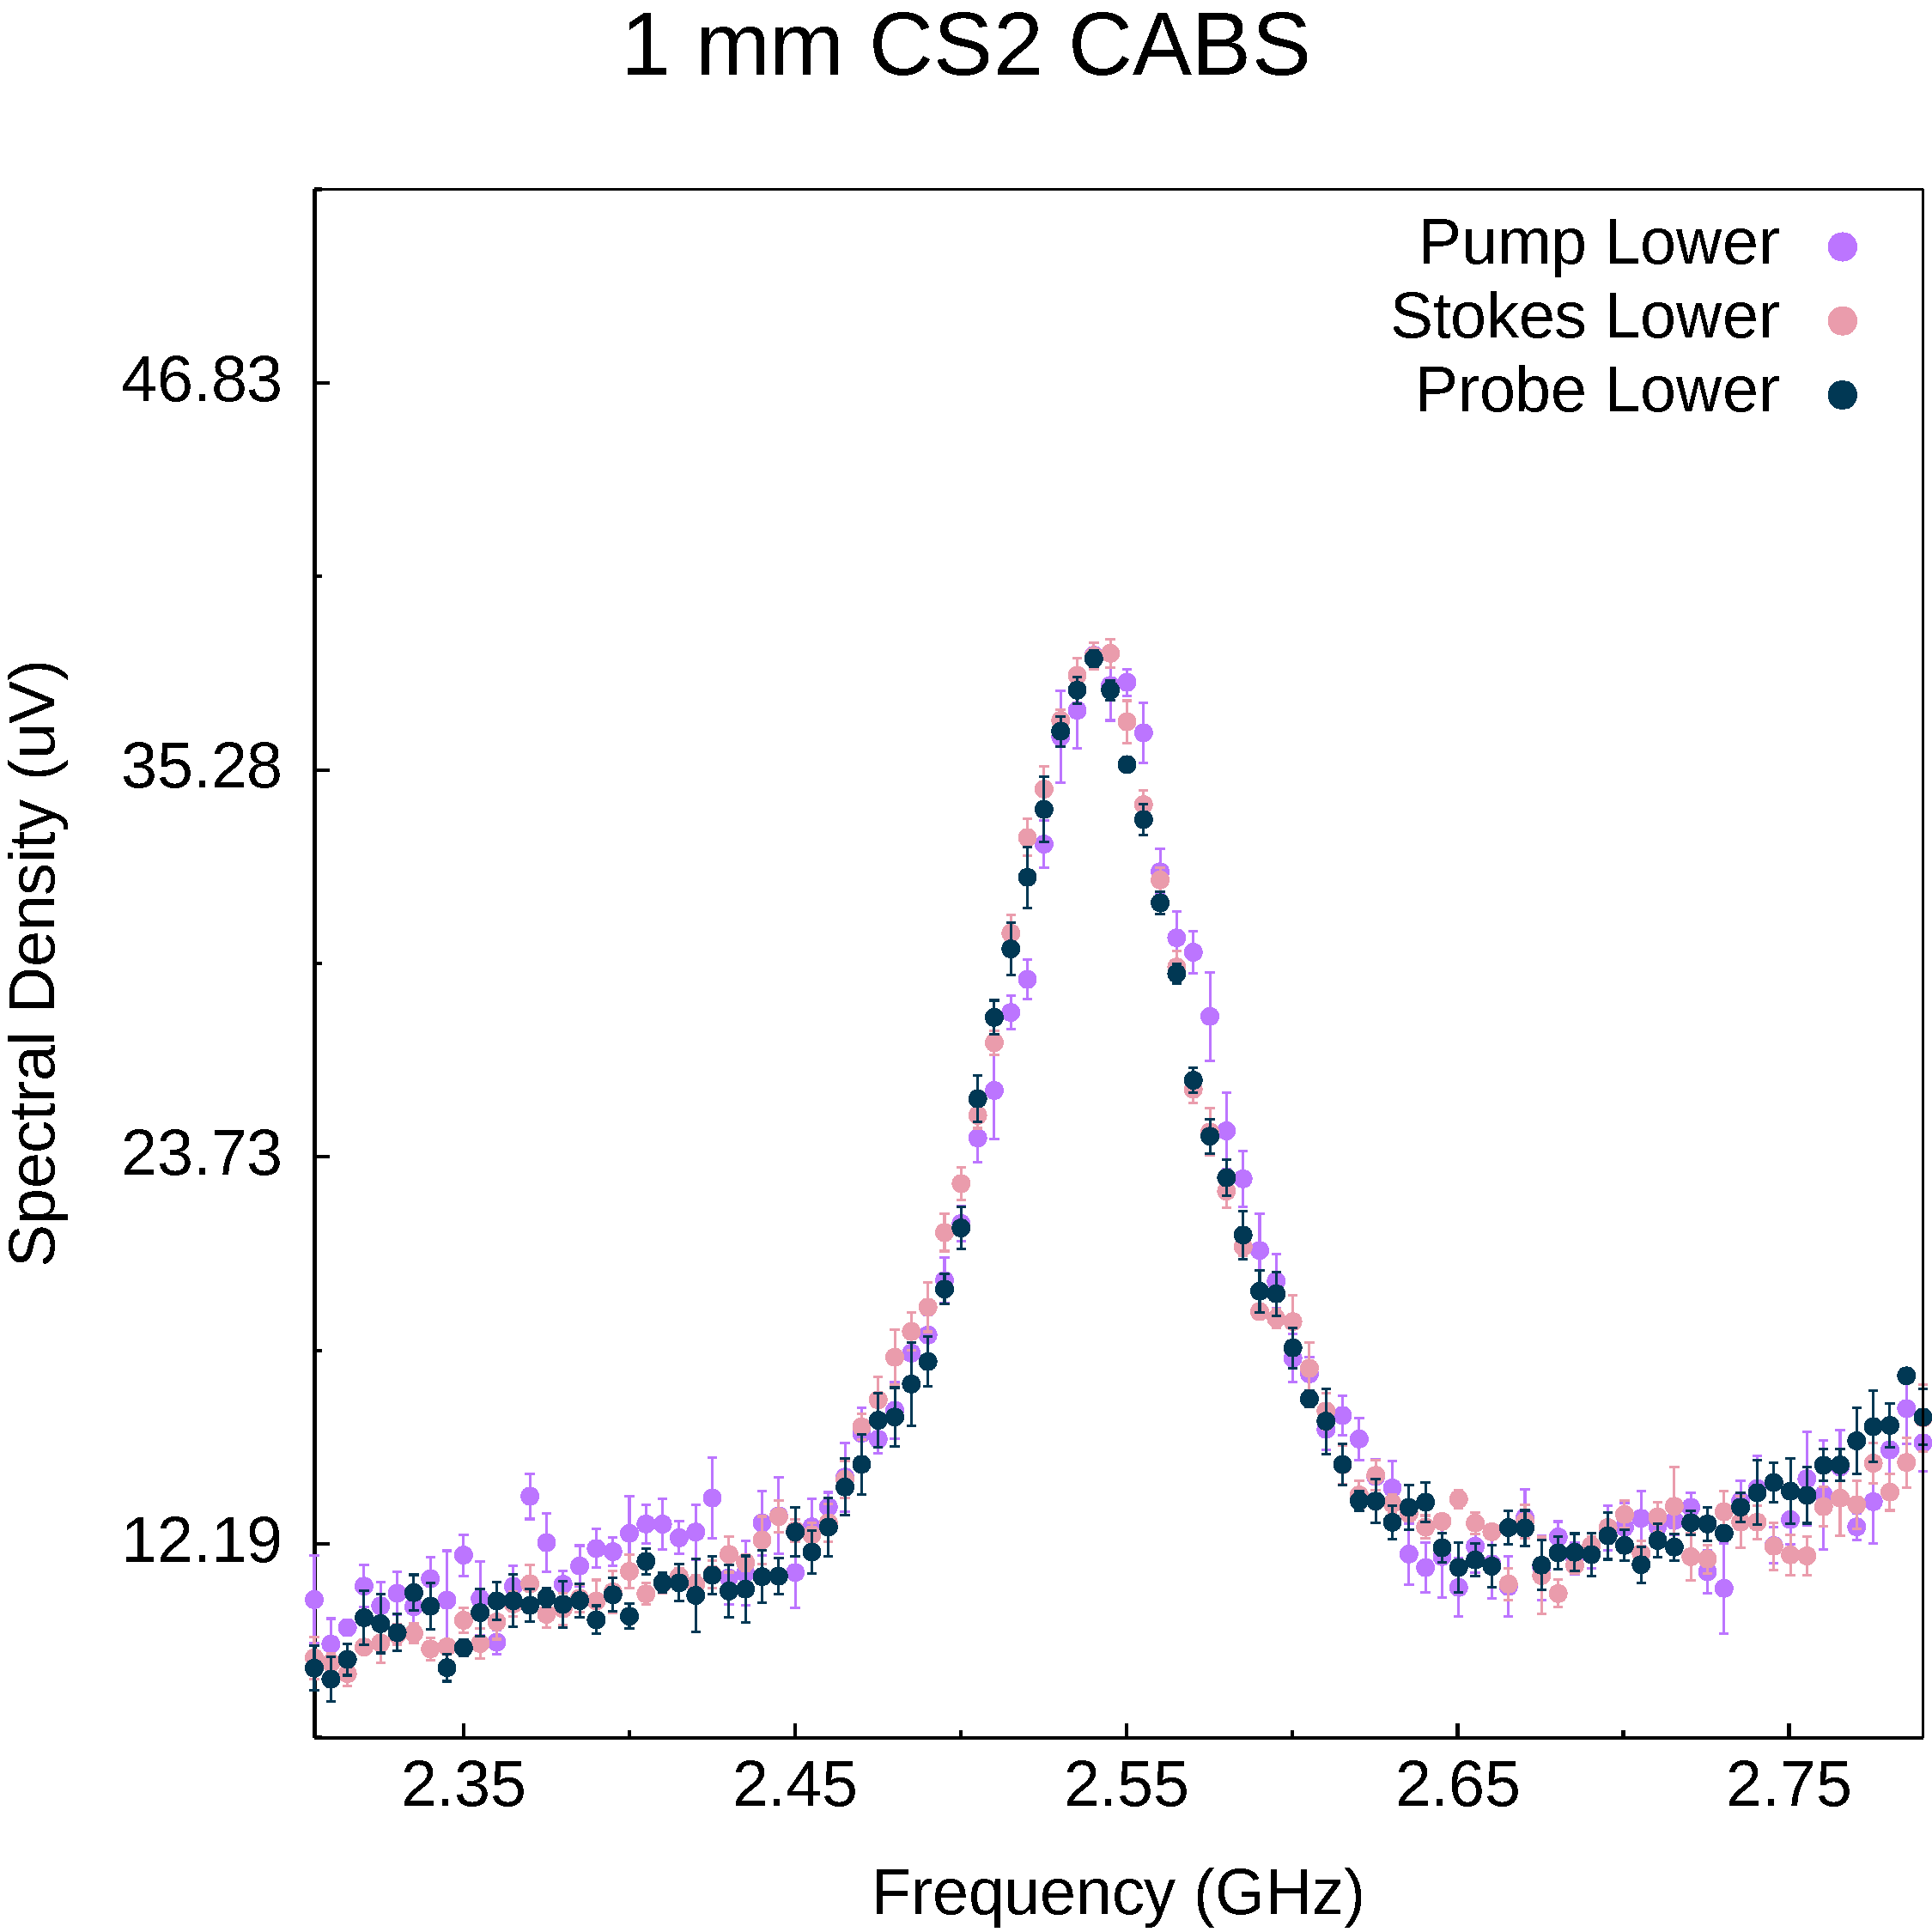
\includegraphics[width=\textwidth]{PSPr-Contribute-Equally.pdf}
    \caption{Signal power contributions with error bars representing one standard deviation of the mean for each measurement.}
    \label{fig:PSPr-Contribute-Equally}
  \end{subfigure}%
  \hfill
  \begin{subfigure}{0.45\textwidth}
    \centering
    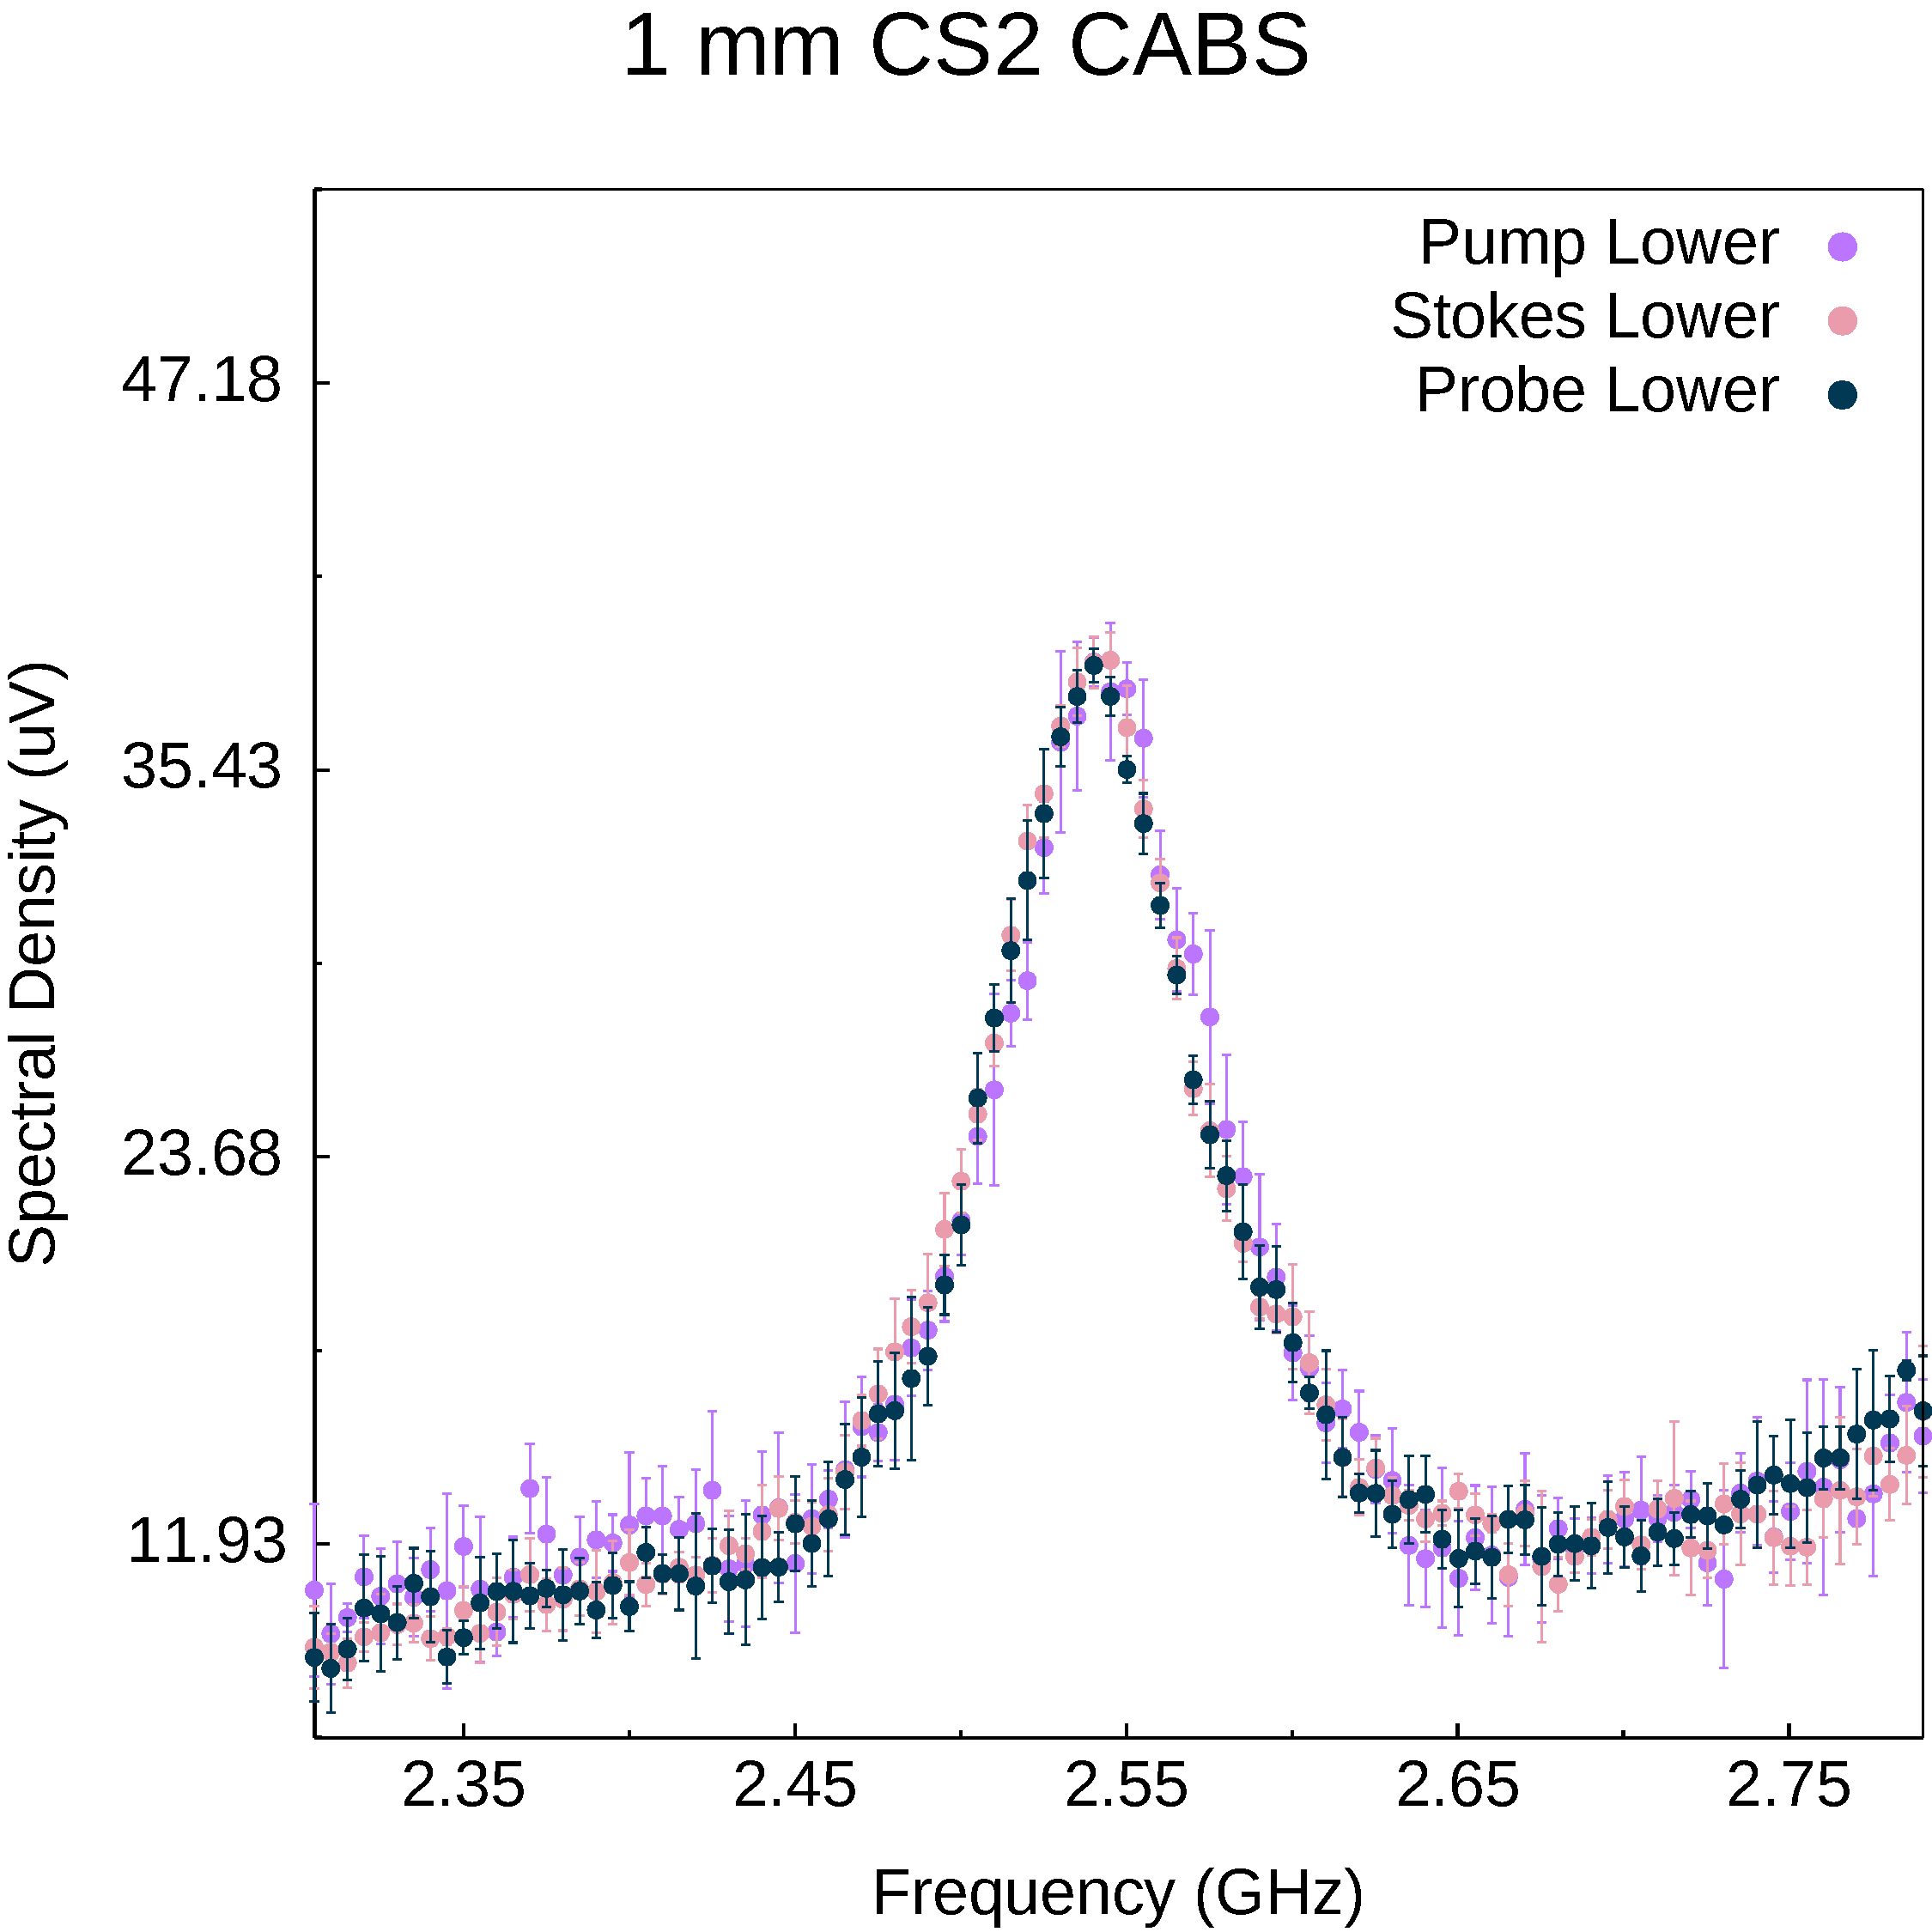
\includegraphics[width=\textwidth]{PSPr-Contribute-Equally-2sigma.pdf}
    \caption{Signal power contributions with error bars extended to two standard deviations of the mean for each measurement.}
    \label{fig:PSPr-Contribute-Equally-2sigma}
  \end{subfigure}
  \caption{Comparison of Signal power contributions with error bars representing one (a) and two (b) standard deviations of the mean for each measurement.}
  \label{fig:combined}
\end{figure}


\twocolumngrid

\bibliography{apssamp}% Produces the bibliography via BibTeX.

\end{document}
%
% ****** End of file apssamp.tex ******
